\chapter{Optimization}
\label{chap:optim}
%=============================================================================

Almost every problem in machine learning begins with a data set $\bm{X}$, a
model $g(\bm{\theta})$ depending on parameters $\bm{\theta}$, and a cost
function $C(\bm{X},g(\bm{\theta}))$ measuring how badly the model explains the
data.  The model is fitted by finding the $\bm{\theta}$ that minimises the
cost.  In Chapter~\ref{chap:lreg} we were fortunate: the cost was quadratic,
its gradient vanished at a point we could write down, and the minimisation
reduced to a linear system.  That good fortune does not survive contact with
logistic regression, and it certainly does not survive neural networks.  For
everything that follows in this book we must find minima numerically.

This chapter builds the tools.  We begin with the question of when a minimum
is worth looking for at all -- convexity -- and with Newton's method, which is
the ideal we shall spend the rest of the chapter approximating cheaply.  We
then develop gradient descent, using linear regression as a test bed precisely
because we already know the answer, and we identify exactly what makes plain
gradient descent slow: the conditioning of the Hessian, a quantity we have
already met twice, in Section~\ref{sec:norms} as a numerical diagnosis and in
Section~\ref{sec:olsstatistics} as a statistical one.  Everything after that --
momentum, stochastic gradients, AdaGrad, RMSProp and Adam -- is an attempt to
defeat that one number without paying the cost of computing the Hessian.

The reader who wants a single organising idea should hold on to this: gradient
descent takes the same step in every direction, but the cost function does not
curve equally in every direction, and the whole art lies in fixing that
mismatch.

%----------------------------------------------------------------------
\section{Convexity}
\label{sec:convexity}

\index{convex function}\index{convex set}
Ideally we want our cost function to be convex, and it is worth stating
precisely what that buys us.

We first need convex sets.  A set $C\subset\mathbb{R}^{n}$ is \emph{convex} if,
for all $\bm{x}$ and $\bm{y}$ in $C$ and all $t\in(0,1)$, the point
$(1-t)\bm{x}+t\bm{y}$ also belongs to $C$; geometrically, every point on the
line segment joining two points of $C$ lies in $C$.  The convex subsets of
$\mathbb{R}$ are the intervals; examples in $\mathbb{R}^{2}$ include the
regular polygons and the discs.

\paragraph{Convex functions.}
Let $X\subset\mathbb{R}^{n}$ be a convex set and $f:X\rightarrow\mathbb{R}$
continuous.  Then $f$ is \emph{convex} if
\begin{equation}
  f\left(t\bm{x}_1+(1-t)\bm{x}_2\right)
   \le t f(\bm{x}_1) + (1-t) f(\bm{x}_2)
  \label{eq:4-convexdef}
\end{equation}
for all $\bm{x}_1,\bm{x}_2\in X$ and all $t\in[0,1]$.  Replacing $\le$ by a
strict inequality, with $\bm{x}_1\neq\bm{x}_2$ and $t\in(0,1)$, defines a
\emph{strictly convex} function.  For a function of one variable the condition
says that the chord joining $f(x_1)$ and $f(x_2)$ lies above the graph on the
whole interval $[x_1,x_2]$.

\paragraph{First-order condition.}
Suppose $f$ is differentiable.  Then $f$ is convex if and only if its domain
$D_f$ is convex and
\begin{equation}
  f(\bm{y}) \ge f(\bm{x}) + \nabla f(\bm{x})^{T}(\bm{y}-\bm{x})
  \label{eq:4-firstorder}
\end{equation}
for all $\bm{x},\bm{y}\in D_f$.  In words: the first-order Taylor expansion at
any point is a global underestimator of the function.  Drawing the tangent to
$f(x)=x^{2}+1$ at any point and observing that it lies everywhere below the
parabola is enough to make the statement believable.

\paragraph{Second-order condition.}
If $f$ is twice differentiable, so that the Hessian exists everywhere, then
$f$ is convex if and only if $D_f$ is convex and the Hessian is positive
semi-definite at every point of $D_f$.  For one variable this reduces to
$f''(x)\ge0$: non-negative curvature everywhere.  This condition is the useful
one in practice, because it gives a procedure rather than a definition.  Proofs
of both conditions may be found in Boyd and Vandenberghe~\cite{boyd2004}.

\paragraph{Why we care.}
The result that matters is the following.

\begin{notebox}
\textbf{Any stationary point of a convex function is a global minimum.}
Let $f$ be convex and differentiable.  Then any $\bm{x}^{*}$ satisfying
$\nabla f(\bm{x}^{*})=\bm{0}$ minimises $f$ globally.
\end{notebox}

The proof is one line from Eq.~(\ref{eq:4-firstorder}): setting
$\bm{x}=\bm{x}^{*}$ makes the gradient term vanish, leaving
$f(\bm{y})\ge f(\bm{x}^{*})$ for every $\bm{y}$.  For a convex cost function,
therefore, we need only find a point where the gradient vanishes and we are
done -- there are no local minima to be trapped in and no saddle points to be
delayed by.

We have already used this twice.  In Section~\ref{sec:hessian} we showed that
the least-squares Hessian is $\bm{H}=\bm{X}^{T}\bm{X}$, positive semi-definite
because $\bm{z}^{T}\bm{X}^{T}\bm{X}\bm{z}=\|\bm{X}\bm{z}\|_2^{2}\ge0$, so the
OLS problem is convex and the normal equations~(\ref{eq:1-normalequations})
deliver the global minimum.  Adding the Ridge penalty makes the Hessian
$\bm{X}^{T}\bm{X}+\lambda\bm{I}$, positive definite for $\lambda>0$, so the
Ridge problem is \emph{strictly} convex and its minimum is unique.  The Lasso
cost of Eq.~(\ref{eq:3-lassoproblem}) is convex but not differentiable, which
is why Section~\ref{sec:lasso} needed coordinate descent rather than a
gradient.

The bad news is that the cost functions of the later chapters are not convex.
A neural network with even one hidden layer has a cost surface with many local
minima, and the guarantee above does not apply.  We shall nonetheless use
methods designed for the convex case, because they work in practice; but it is
important to know that when we do so we are relying on empirical good
behaviour rather than on a theorem.

%----------------------------------------------------------------------
\section{Newton's method}
\label{sec:newton}

\index{Newton-Raphson method}
Before descending gradients it is worth recalling the method that uses
curvature properly, both because it is the standard against which everything
else is measured and because its cost is what motivates the alternatives.

\paragraph{Root finding in one dimension.}
Newton's method, also called Newton-Raphson, finds a root of $f$ by extending
the tangent line at the current point until it crosses zero.  Taylor expanding
about a point $x$ close to the solution $s$,
\begin{equation}
  f(s) = 0 = f(x) + (s-x)f'(x) + \frac{(s-x)^{2}}{2}f''(x)+\dots,
  \label{eq:4-taylornr}
\end{equation}
and discarding terms beyond the linear one gives $f(x)+(s-x)f'(x)\approx0$,
that is $s\approx x-f(x)/f'(x)$.  As an iteration,
\begin{equation}
  x_{n+1} = x_n - \frac{f(x_n)}{f'(x_n)} .
  \label{eq:4-newton1d}
\end{equation}
Geometrically $x_{n+1}$ is where the tangent at $(x_n,f(x_n))$ meets the
horizontal axis.  Close to a root the convergence is quadratic and extremely
fast.  Far from one, where the discarded terms matter, the formula can be
grossly inaccurate: if an iterate lands near a local extremum, so that
$f'$ nearly vanishes, the method can fail completely.  If the derivative is
available only numerically, or the function is not smooth, Newton's method is
best avoided.

\paragraph{Several variables.}
For a system $f_1(x_1,x_2)=0$, $f_2(x_1,x_2)=0$, Taylor expansion gives
\begin{equation}
  0 = f_k(x_1+h_1,x_2+h_2)
    = f_k(x_1,x_2) + h_1\frac{\partial f_k}{\partial x_1}
                   + h_2\frac{\partial f_k}{\partial x_2} + \dots,
  \qquad k=1,2,
  \label{eq:4-newtonmulti}
\end{equation}
and collecting the partial derivatives into the Jacobian
matrix~(\ref{eq:1-jacobian}),
\begin{equation}
  \bm{J} = \begin{pmatrix}
    \partial f_1/\partial x_1 & \partial f_1/\partial x_2\\
    \partial f_2/\partial x_1 & \partial f_2/\partial x_2
  \end{pmatrix},
  \label{eq:4-jacobian2}
\end{equation}
the update becomes $\bm{x}^{n+1}=\bm{x}^{n}+\bm{h}^{n}$ with
\begin{equation}
  \bm{h}^{n} = -\bm{J}^{-1}\bm{f}(\bm{x}^{n}).
  \label{eq:4-newtonstep}
\end{equation}
We must invert the Jacobian, and difficulties arise when it is nearly
singular -- the conditioning problem of Section~\ref{sec:norms} again.

\paragraph{Newton's method for minimisation.}
Minimising $C(\bm{\theta})$ means finding a root of $\nabla C$, so we apply the
above with $\bm{f}=\nabla C$.  The Jacobian of the gradient is the Hessian,
and the iteration reads
\begin{equation}
  \boxed{\;
  \bm{\theta}_{k+1} = \bm{\theta}_k
    - \bm{H}^{-1}(\bm{\theta}_k)\,\nabla C(\bm{\theta}_k) . \;}
  \label{eq:4-newtonopt}
\end{equation}
Equation~(\ref{eq:4-newtonopt}) is the ideal against which the rest of this
chapter should be read.  It is what one gets by minimising the second-order
Taylor expansion of the cost exactly, and it has two properties no
gradient-only method can match: it converges quadratically near the minimum,
and it is \emph{invariant} under linear rescaling of the parameters, so that
the conditioning problems which dominate everything below simply do not arise.

Applied to ordinary least squares it is not merely fast but exact.  With
$\nabla C=-2\bm{X}^{T}(\bm{y}-\bm{X}\bm{\theta})/n$ from
Eq.~(\ref{eq:1-olsgradient}) and $\bm{H}=2\bm{X}^{T}\bm{X}/n$ from
Eq.~(\ref{eq:1-hessian}), a single step from any starting point gives
\begin{equation}
  \bm{\theta}_{1} = \bm{\theta}_0
    + \left(\bm{X}^{T}\bm{X}\right)^{-1}\bm{X}^{T}
      \left(\bm{y}-\bm{X}\bm{\theta}_0\right)
    = \left(\bm{X}^{T}\bm{X}\right)^{-1}\bm{X}^{T}\bm{y},
  \label{eq:4-newtonols}
\end{equation}
the exact solution~(\ref{eq:3-olssolution}).  This is not a coincidence: for a
quadratic cost the second-order Taylor expansion is the function itself, so
one Newton step lands on the minimum.

\paragraph{Why we do not simply use it.}
For $p$ parameters the Hessian has $p^{2}$ entries and inverting it costs
$\bigO(p^{3})$ operations by Section~\ref{sec:lu}.  For a linear regression
with twenty features this is nothing.  For a neural network with $10^{7}$
parameters the Hessian would need $10^{14}$ numbers, which cannot be stored,
let alone factorised.  The entire subject of this chapter is the construction
of methods that capture some of the benefit of Eq.~(\ref{eq:4-newtonopt}) at a
cost linear rather than cubic in $p$.

%----------------------------------------------------------------------
\section{Gradient descent}
\label{sec:graddescent}

\index{gradient descent}\index{steepest descent}
The basic idea is that a function $F(\bm{x})$ decreases fastest, locally, if
one moves from $\bm{x}$ in the direction of the negative gradient
$-\nabla F(\bm{x})$.  One can show that for
\begin{equation}
  \bm{x}_{k+1} = \bm{x}_k - \gamma_k\nabla F(\bm{x}_k),
  \qquad \gamma_k>0,
  \label{eq:4-gd}
\end{equation}
and for $\gamma_k$ small enough, $F(\bm{x}_{k+1})\le F(\bm{x}_k)$: we always
move towards smaller function values.  Iterating Eq.~(\ref{eq:4-gd}) from an
initial guess $\bm{x}_0$ is the method of \emph{steepest descent}, or simply
\emph{gradient descent} (GD).  The parameter $\gamma_k$ is the step length, or
in machine learning the \emph{learning rate}.  We use the symbol $\gamma$
for it throughout this book, with a subscript when it changes from one
iteration to the next.

Ideally the sequence converges to a global minimum.  In general we do not know
whether a minimum we reach is global or local; but by
Section~\ref{sec:convexity}, if $F$ is convex the question does not arise.  The
scheme is conceptually simple and easy to implement.  It also has severe
limitations.

\paragraph{Limitations.}
In machine learning we are often faced with non-convex, high-dimensional cost
functions with many local minima.  Gradient descent is deterministic, so
unless the initial guess is good it will descend into whichever local minimum
it happens to face, and the result is sensitive to that initial condition.
The gradient is a function of all $p$ parameters and can be expensive to
evaluate.  And the method is delicate in its dependence on $\gamma$: we are
guaranteed $F(\bm{x}_{k+1})\le F(\bm{x}_k)$ only for sufficiently small steps,
so too large a value produces erratic behaviour or divergence while too small
a value converges intolerably slowly.  Determining a good $\gamma$ is the
central practical difficulty, and Sections~\ref{sec:adagrad} to
\ref{sec:adam} are devoted to removing the need to do so by hand.

Many of these shortcomings can be alleviated by introducing randomness, which
is the subject of Section~\ref{sec:sgd}.

%----------------------------------------------------------------------
\section{Gradient descent for linear regression}
\label{sec:gdlinreg}

\index{gradient descent!for least squares}
Linear regression is the ideal test case for gradient descent, for three
reasons: it has an analytical solution to check against, its gradient can be
computed exactly, and its cost function is convex so that convergence is
guaranteed for small enough learning rates.

We take the data set used throughout Chapter~\ref{chap:lreg},
\begin{equation*}
  y_i = 4 + 3x_i + \varepsilon_i,
  \qquad x_i \sim \mathcal{U}(0,2),
  \qquad \varepsilon_i\sim\mathcal{N}(0,1),
\end{equation*}
with $n=100$ points, and the design matrix including an intercept column,
\begin{equation}
  \bm{X} = \begin{bmatrix}
    1 & x_0\\ \vdots & \vdots\\ 1 & x_{n-1}
  \end{bmatrix}
  \in\mathbb{R}^{n\times2},
  \qquad
  \bm{\theta}=\begin{pmatrix}\theta_0\\\theta_1\end{pmatrix}.
  \label{eq:4-gddesign}
\end{equation}
The cost function is
\begin{equation}
  C(\bm{\theta}) = \frac{1}{n}\left\|\bm{X}\bm{\theta}-\bm{y}\right\|_2^{2}
   = \frac{1}{n}\sum_{i=0}^{n-1}
     \left[(\theta_0+\theta_1 x_i)^{2}
       -2y_i(\theta_0+\theta_1x_i)+y_i^{2}\right].
  \label{eq:4-gdcost}
\end{equation}
Computing $\partial C/\partial\theta_0$ and $\partial C/\partial\theta_1$
separately and reassembling,
\begin{equation}
  \nabla_{\bm{\theta}}C(\bm{\theta})
   = \frac{2}{n}\begin{bmatrix}
       \sum_i\left(\theta_0+\theta_1x_i-y_i\right)\\
       \sum_i\left(x_i(\theta_0+\theta_1x_i)-y_ix_i\right)
     \end{bmatrix}
   = \frac{2}{n}\bm{X}^{T}\left(\bm{X}\bm{\theta}-\bm{y}\right),
  \label{eq:4-gdgradient}
\end{equation}
which is Eq.~(\ref{eq:1-olsgradient}) written out coordinate by coordinate.
The Hessian is
\begin{equation}
  \bm{H} = \begin{bmatrix}
    \dfrac{\partial^{2}C}{\partial\theta_0^{2}} &
    \dfrac{\partial^{2}C}{\partial\theta_0\partial\theta_1}\\[8pt]
    \dfrac{\partial^{2}C}{\partial\theta_0\partial\theta_1} &
    \dfrac{\partial^{2}C}{\partial\theta_1^{2}}
  \end{bmatrix}
   = \frac{2}{n}\bm{X}^{T}\bm{X},
  \label{eq:4-gdhessian}
\end{equation}
in agreement with Eq.~(\ref{eq:1-hessian}), and positive semi-definite, so
$C$ is convex and any stationary point is the global minimum.

The gradient descent iteration is
\begin{equation}
  \bm{\theta}_{k+1} = \bm{\theta}_k - \gamma\,\nabla_{\bm{\theta}}C(\bm{\theta}_k),
  \qquad k=0,1,\dots
  \label{eq:4-gditeration}
\end{equation}
started from a random $\bm{\theta}_0$ and stopped when
$\|\nabla_{\bm{\theta}}C\|\le\epsilon$ for some tolerance, say $10^{-8}$.

\begin{Python}{}
import numpy as np

n = 100
rng = np.random.default_rng(2024)
x = 2.0 * rng.random((n, 1))
y = 4.0 + 3.0 * x + rng.normal(size=(n, 1))
X = np.c_[np.ones((n, 1)), x]

# The analytical solution of Chapter 3, for comparison
theta_exact = np.linalg.pinv(X.T @ X) @ X.T @ y
print("analytical:", theta_exact.ravel())

# Gradient descent, Eq. (4.gditeration)
theta = rng.normal(size=(2, 1))
gamma = 0.1
for k in range(1000):
    gradient = (2.0 / n) * X.T @ (X @ theta - y)
    theta -= gamma * gradient
    if np.linalg.norm(gradient) < 1.0e-8:
        break
print(f"gradient descent after {k+1} iterations:", theta.ravel())
\end{Python}

With $\gamma=0.1$ the iteration reproduces the analytical answer to five decimal
places within a few hundred steps.  With $\gamma=0.001$, the value used in the
lecture notes, a thousand iterations are not nearly enough; with
$\gamma$ too large it diverges.  The next section explains exactly where the
boundary lies.

%......................................................................
\subsection{Gradient descent for Ridge regression}
\label{sec:gdridge}

The same treatment applies to the Ridge cost of Eq.~(\ref{eq:3-ridgeproblem}).
Writing it as
\begin{equation}
  C(\bm{\theta}) = \frac{1}{n}\left\|\bm{X}\bm{\theta}-\bm{y}\right\|_2^{2}
                 + \lambda\bm{\theta}^{T}\bm{\theta},
  \label{eq:4-ridgecost}
\end{equation}
the gradient and Hessian follow from
Eqs.~(\ref{eq:1-dlinear}) and (\ref{eq:1-dquadsym}),
\begin{equation}
  \nabla_{\bm{\theta}}C
   = \frac{2}{n}\bm{X}^{T}\left(\bm{X}\bm{\theta}-\bm{y}\right)
     + 2\lambda\bm{\theta},
  \qquad
  \bm{H} = \frac{2}{n}\bm{X}^{T}\bm{X} + 2\lambda\bm{I} .
  \label{eq:4-ridgegradhess}
\end{equation}
Setting the gradient to zero returns the closed
form~(\ref{eq:3-ridgesolution}), as it must.  The Hessian is now positive
definite for every $\lambda>0$, so the problem is strictly convex.

\begin{Python}{}
import numpy as np

lmbda = 0.001
theta = rng.normal(size=(2, 1))
gamma = 0.1
for k in range(1000):
    gradient = 2.0 * (X.T @ (X @ theta - y) / n + lmbda * theta)
    theta -= gamma * gradient

# Compare with the closed form of Chapter 3
I = np.eye(X.shape[1])
theta_exact = np.linalg.inv(X.T @ X + n * lmbda * I) @ X.T @ y
print("gradient descent:", theta.ravel())
print("closed form:     ", theta_exact.ravel())
\end{Python}

Note the factor $n$ in the closed form.  Our cost~(\ref{eq:4-ridgecost})
carries $1/n$ on the data term but not on the penalty, whereas
Eq.~(\ref{eq:3-ridgesolution}) was derived with neither; the two agree only if
$\lambda$ is scaled accordingly.  This is precisely the class of bookkeeping
error warned against in Section~\ref{sec:scalingintercept}, and it is worth
tracking carefully whenever a penalised gradient is implemented.

%----------------------------------------------------------------------
\section{The learning rate and the condition number}
\label{sec:learningrate}

\index{learning rate}\index{condition number!and gradient descent}
We can now answer the question of how large $\gamma$ may be, and in doing so
identify the quantity that governs everything in the rest of this chapter.

Consider a quadratic cost with symmetric positive definite Hessian $\bm{H}$,
which by Eq.~(\ref{eq:4-gdhessian}) is the case for least squares.  Write the
error at step $k$ as $\bm{e}_k=\bm{\theta}_k-\bm{\theta}^{*}$, with
$\bm{\theta}^{*}$ the minimum.  Since $\nabla C(\bm{\theta})=\bm{H}\bm{e}$ for
a quadratic, the iteration~(\ref{eq:4-gditeration}) gives
\begin{equation}
  \bm{e}_{k+1} = \bm{e}_k - \gamma\bm{H}\bm{e}_k
               = \left(\bm{I}-\gamma\bm{H}\right)\bm{e}_k .
  \label{eq:4-errorrecursion}
\end{equation}
Now diagonalise.  By the spectral decomposition~(\ref{eq:1-spectral}),
$\bm{H}=\bm{Q}\bm{\Lambda}\bm{Q}^{T}$ with orthonormal eigenvectors and
eigenvalues $\lambda_i>0$.  Expressing the error in the eigenbasis,
$\tilde{\bm{e}}=\bm{Q}^{T}\bm{e}$, and multiplying
Eq.~(\ref{eq:4-errorrecursion}) from the left by $\bm{Q}^{T}$,
\begin{equation*}
  \tilde{\bm{e}}_{k+1}
   = \bm{Q}^{T}\left(\bm{I}-\gamma\bm{H}\right)\bm{Q}\,\tilde{\bm{e}}_k
   = \left(\bm{I}-\gamma\bm{\Lambda}\right)\tilde{\bm{e}}_k ,
\end{equation*}
because $\bm{Q}^{T}\bm{Q}=\bm{I}$ and $\bm{Q}^{T}\bm{H}\bm{Q}=\bm{\Lambda}$.
The matrix on the right is diagonal, so the recursion \emph{decouples
completely} into $p$ independent scalar recursions:
\begin{equation}
  \tilde{e}_{k+1,i} = \left(1-\gamma\lambda_i\right)\tilde{e}_{k,i},
  \qquad\text{so}\qquad
  \tilde{e}_{k,i} = \left(1-\gamma\lambda_i\right)^{k}\tilde{e}_{0,i} .
  \label{eq:4-decoupled}
\end{equation}
Each eigendirection contracts by its own factor $|1-\gamma\lambda_i|$ at every
step, and this single equation contains everything.

\paragraph{Stability.}
\index{gradient descent!stability bound}\index{spectral radius}
We can now state and prove the condition on the learning rate.

\begin{theorem}[Stability of gradient descent on a quadratic]
\label{thm:4-gdstability}
Let $\bm{H}$ be symmetric positive definite with eigenvalues
$0<\lambda_{\min}\le\lambda_i\le\lambda_{\max}$.  The gradient descent
iteration~(\ref{eq:4-gditeration}) with fixed learning rate $\gamma$ converges
to $\bm{\theta}^{*}$ from every starting point $\bm{\theta}_0$ if and only if
\begin{equation}
  \boxed{\;0 < \gamma < \frac{2}{\lambda_{\max}} \;}
  \label{eq:4-stability}
\end{equation}
Equivalently, the spectral radius of the iteration matrix satisfies
\begin{equation}
  \rho\!\left(\bm{I}-\gamma\bm{H}\right)
   = \max_i\left|1-\gamma\lambda_i\right| < 1 .
  \label{eq:4-spectralradius}
\end{equation}
\end{theorem}

\begin{proof}
By Eq.~(\ref{eq:4-decoupled}) the $i$-th component of the error in the
eigenbasis is $\tilde{e}_{k,i}=(1-\gamma\lambda_i)^{k}\tilde{e}_{0,i}$, a
geometric sequence with ratio $1-\gamma\lambda_i$.  It tends to zero for
every $\tilde{e}_{0,i}$ precisely when $|1-\gamma\lambda_i|<1$.  Since
$\lambda_i>0$ we may unpack the absolute value:
\begin{equation*}
  -1 < 1-\gamma\lambda_i < 1
  \quad\Longleftrightarrow\quad
  -2 < -\gamma\lambda_i < 0
  \quad\Longleftrightarrow\quad
  0 < \gamma < \frac{2}{\lambda_i} .
\end{equation*}
Because $\bm{Q}$ is orthogonal, $\|\bm{e}_k\|=\|\tilde{\bm{e}}_k\|$, so
$\bm{e}_k\to\bm{0}$ for every $\bm{e}_0$ if and only if every component
converges, that is
\begin{equation*}
  0 < \gamma < \min_i\frac{2}{\lambda_i} = \frac{2}{\lambda_{\max}} ,
\end{equation*}
since $2/\lambda_i$ is smallest for the largest eigenvalue.  This is
Eq.~(\ref{eq:4-stability}).  For the converse, suppose
$\gamma\ge2/\lambda_{\max}$ and take $\bm{e}_0$ with a non-zero component along
the eigenvector of $\lambda_{\max}$; that component has
$|1-\gamma\lambda_{\max}|\ge1$ and does not decay, so the iteration fails to
converge from this $\bm{\theta}_0$.  Finally, the eigenvalues of
$\bm{I}-\gamma\bm{H}$ are $1-\gamma\lambda_i$ (the eigenvectors are those of
$\bm{H}$), so its spectral radius is $\max_i|1-\gamma\lambda_i|$, and the
condition just derived is exactly Eq.~(\ref{eq:4-spectralradius}).
\end{proof}

The bound is set by the \emph{steepest} direction, whatever the others are
doing: the direction of greatest curvature is the one along which a gradient
step changes the parameters most, and it is therefore the first to become
unstable.  Exceed the bound and the component along that direction grows
geometrically; this is the divergence one observes when the learning rate is
set too high.

\paragraph{At and beyond the bound.}
It is worth reading off from Eq.~(\ref{eq:4-decoupled}) exactly what the
stiffest mode does as $\gamma$ increases.  Its multiplier is
$1-\gamma\lambda_{\max}$, so for $0<\gamma<1/\lambda_{\max}$ the mode decays
monotonically without changing sign; for
$1/\lambda_{\max}<\gamma<2/\lambda_{\max}$ the multiplier is negative and the
mode alternates in sign at every step while its magnitude still decreases --
this is the zig-zag across the valley in the centre panel of
Figure~\ref{fig:gdpaths}; at $\gamma=2/\lambda_{\max}$ the multiplier is
exactly $-1$ and the mode oscillates forever without decaying; and for
$\gamma>2/\lambda_{\max}$ the multiplier has magnitude greater than one and
the mode diverges.  The strict inequality in Eq.~(\ref{eq:4-stability}) is
therefore essential: at the boundary itself nothing blows up, but nothing
converges either.

\paragraph{Decrease of the cost.}
The same calculation shows that, inside the stable range, the cost itself
decreases at every step and not only the error.  For a quadratic with
Hessian $\bm{H}$ the excess cost is
$C(\bm{\theta})-C(\bm{\theta}^{*})=\tfrac12\bm{e}^{T}\bm{H}\bm{e}$, which
in the eigenbasis reads
\begin{align}
  C(\bm{\theta}_k)-C(\bm{\theta}^{*})
   &= \frac12\sum_{i=1}^{p}\lambda_i\,\tilde{e}_{k,i}^{2},
  \nonumber\\
  C(\bm{\theta}_{k+1})-C(\bm{\theta}^{*})
   &= \frac12\sum_{i=1}^{p}\lambda_i\left(1-\gamma\lambda_i\right)^{2}
     \tilde{e}_{k,i}^{2} .
  \label{eq:4-lossmodes}
\end{align}
Every non-zero term shrinks when $(1-\gamma\lambda_i)^{2}<1$, which is the
condition of the theorem once more.  Hence Eq.~(\ref{eq:4-stability})
guarantees a strict reduction of the cost at every iterate that is not
already the minimum.  (For least squares $\bm{H}=2\bm{X}^{T}\bm{X}/n$, and
one checks directly that
$C(\bm{\theta})-C(\bm{\theta}^{*})=\|\bm{X}\bm{e}\|^{2}/n
=\tfrac12\bm{e}^{T}\bm{H}\bm{e}$.)

\paragraph{Beyond quadratics.}
\index{Lipschitz continuity!of the gradient}\index{descent lemma}
Nothing in the argument used that the cost was a quadratic \emph{globally}.
Near a minimum $\bm{\theta}^{*}$ of any twice differentiable cost,
$\nabla C(\bm{\theta}^{*})=\bm{0}$ and Taylor expansion gives
$\nabla C(\bm{\theta})=\bm{H}^{*}\bm{e}+\mathcal{O}(\|\bm{e}\|^{2})$ with
$\bm{H}^{*}=\nabla^{2}C(\bm{\theta}^{*})$, so the recursion
(\ref{eq:4-errorrecursion}) describes the local dynamics and the theorem
gives the local stability condition, with $\lambda_{\max}$ the largest
eigenvalue of the Hessian \emph{at the minimum}.  A global statement needs a
global bound on the curvature.  Suppose the gradient is Lipschitz continuous
with constant $L$,
\begin{equation}
  \left\|\nabla C(\bm{\theta})-\nabla C(\bm{\theta}')\right\|
   \le L\left\|\bm{\theta}-\bm{\theta}'\right\|
  \qquad\text{for all }\bm{\theta},\bm{\theta}' ,
  \label{eq:4-lipschitz}
\end{equation}
which for a twice differentiable cost means that all Hessian eigenvalues lie
in $[-L,L]$ everywhere.  Then the \emph{descent lemma} holds: for any
$\bm{\theta}$ and any step $\bm{d}$,
\begin{equation}
  C(\bm{\theta}+\bm{d})
   \le C(\bm{\theta})+\nabla C(\bm{\theta})^{T}\bm{d}+\frac{L}{2}\|\bm{d}\|^{2}.
  \label{eq:4-descentlemma}
\end{equation}
To see this, write the change in the cost as an integral along the segment
from $\bm{\theta}$ to $\bm{\theta}+\bm{d}$ and subtract and add
$\nabla C(\bm{\theta})^{T}\bm{d}$ under the integral sign,
\begin{align*}
  C(\bm{\theta}+\bm{d})-C(\bm{\theta})
   &= \int_0^1\nabla C(\bm{\theta}+t\bm{d})^{T}\bm{d}\,dt\\
   &= \nabla C(\bm{\theta})^{T}\bm{d}
     +\int_0^1\left[\nabla C(\bm{\theta}+t\bm{d})-\nabla C(\bm{\theta})\right]^{T}
      \bm{d}\,dt ;
\end{align*}
the Cauchy--Schwarz inequality and Eq.~(\ref{eq:4-lipschitz}) bound the
integrand by $Lt\|\bm{d}\|^{2}$, and $\int_0^1 Lt\,dt=L/2$.  Taking the
gradient step $\bm{d}=-\gamma\bm{g}_k$ with $\bm{g}_k=\nabla C(\bm{\theta}_k)$,
\begin{align}
  C(\bm{\theta}_{k+1})
   &\le C(\bm{\theta}_k)-\gamma\|\bm{g}_k\|^{2}
       +\frac{L\gamma^{2}}{2}\|\bm{g}_k\|^{2}
  \nonumber\\
   &= C(\bm{\theta}_k)-\gamma\left(1-\frac{L\gamma}{2}\right)\|\bm{g}_k\|^{2},
  \label{eq:4-Lbound}
\end{align}
so the cost decreases strictly, wherever the gradient is non-zero, whenever
\begin{equation*}
  0<\gamma<\frac{2}{L}.
\end{equation*}
This is the ``sufficiently small step'' promised in
Section~\ref{sec:graddescent}, now made quantitative.  For a quadratic the
Lipschitz constant of the gradient is $L=\lambda_{\max}(\bm{H})$, and the
descent lemma reproduces the stability bound~(\ref{eq:4-stability}) exactly.

\paragraph{Qualifications.}
Four remarks delimit what has been proved.  Positive definiteness matters:
if $\bm{H}$ has a negative eigenvalue, the corresponding multiplier
$1-\gamma\lambda_i$ exceeds one for every $\gamma>0$ and no fixed positive
learning rate contracts that direction -- gradient descent moves away from a
saddle point or a maximum, which is what one wants, but the analysis above no
longer describes convergence.  If $\bm{H}$ has zero eigenvalues, the
multiplier along the corresponding flat directions is exactly one and the
quadratic model predicts no contraction at all; for least squares this is the
rank-deficient case of Section~\ref{sec:ridgesvd}, and the remedy is the
Ridge penalty discussed below.  For a non-quadratic cost the eigenvalues vary
with $\bm{\theta}$: the local bound uses the Hessian at the minimum, whereas a
global guarantee needs a Lipschitz constant $L$ valid over the whole region
visited by the iterates, which is typically much larger and makes the
permitted step correspondingly smaller.  And stochastic gradients, the
subject of Section~\ref{sec:sgd}, add noise to every step, so the
deterministic bound is a guide to stability rather than a complete
convergence theory.

\paragraph{Speed.}
Inside the stable range the question becomes how fast the error contracts,
and the answer is set by the two extreme eigenvalues.  The worst-case
contraction factor per step is
\begin{equation*}
  r(\gamma)=\max_i\left|1-\gamma\lambda_i\right|
          =\max\left\{\,\left|1-\gamma\lambda_{\min}\right|,\;
                        \left|1-\gamma\lambda_{\max}\right|\,\right\},
\end{equation*}
because $|1-\gamma\lambda|$ is largest at one end or the other of the
spectrum.  For $\gamma\le1/\lambda_{\max}$ the first term dominates and
$r$ decreases with $\gamma$; for larger $\gamma$ the second term
$\gamma\lambda_{\max}-1$ grows.  The minimum lies where the two are equal,
$1-\gamma\lambda_{\min}=\gamma\lambda_{\max}-1$, which gives the optimal
learning rate $\gamma^{*}=2/(\lambda_{\max}+\lambda_{\min})$ and the
contraction rate
\begin{equation}
  \left|\frac{\lambda_{\max}-\lambda_{\min}}{\lambda_{\max}+\lambda_{\min}}\right|
   = \frac{\kappa-1}{\kappa+1},
  \qquad
  \kappa = \frac{\lambda_{\max}}{\lambda_{\min}} = \kappa_2(\bm{H}),
  \label{eq:4-gdrate}
\end{equation}
where $\kappa$ is the condition number of the Hessian in the sense of
Eq.~(\ref{eq:1-cond2}).  Since $(\kappa-1)/(\kappa+1)\approx1-2/\kappa$ for
large $\kappa$, the number of iterations needed to reduce the error by a fixed
factor is proportional to $\kappa$: a large condition number produces slow
convergence even when the learning rate is perfectly stable and optimally
chosen.

Figure~\ref{fig:etabound} confirms both statements numerically.  The
iteration count falls as $\gamma$ increases, reaches its minimum at the predicted
$\gamma^{*}=2/(\lambda_{\max}+\lambda_{\min})$, rises again, and diverges
exactly at $2/\lambda_{\max}$.  There is no margin of safety at the right-hand
edge: the transition from the fastest convergence available to outright
divergence occupies a factor of two in $\gamma$.

\begin{figure}[htbp]
\centering
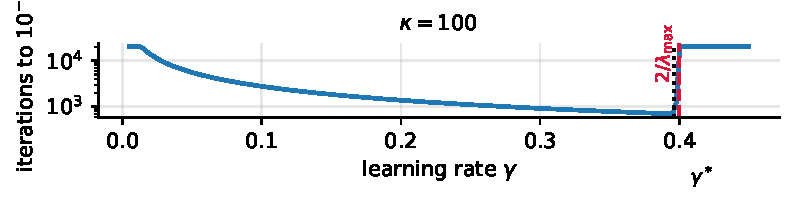
\includegraphics[width=0.62\textwidth]{BookFigures/chapter04_optimization/learning_rate_bound}
\caption{Iterations required to reach an error of $10^{-6}$ against the learning rate, for a quadratic with eigenvalues $\{0.05,1,5\}$.  The optimum lies at $\gamma^{*}$ and the method diverges beyond $2/\lambda_{\max}$, as predicted by Eqs.~(\ref{eq:4-stability}) and (\ref{eq:4-gdrate}).}
\label{fig:etabound}
\end{figure}


This is the central result of the chapter, and it deserves to be read slowly.
Gradient descent is not slow because gradients are a bad idea.  It is slow
because it applies \emph{the same} $\gamma$ to every eigendirection, while
stability forces that single $\gamma$ to be dictated by the steepest direction.
In a problem where $\lambda_{\max}/\lambda_{\min}=1000$, the step that is
barely stable along the steep direction is a thousand times too small along
the flat one, and the flat direction is where the remaining error lives.  The
iterates oscillate across the narrow valley while creeping along its floor.

\paragraph{What this means for regression.}
For least squares $\bm{H}=2\bm{X}^{T}\bm{X}/n$, so by
Eq.~(\ref{eq:1-condsquared})
\begin{equation}
  \kappa(\bm{H}) = \kappa_2\left(\bm{X}^{T}\bm{X}\right)
                 = \kappa_2(\bm{X})^{2} ,
  \label{eq:4-kappasquared}
\end{equation}
and the iteration count scales with the \emph{square} of the condition number
of the design matrix.  Three consequences follow, each connecting to earlier
chapters.

First, standardising the features is not only the statistical convention of
Section~\ref{sec:scalingintercept} but a direct accelerator: it makes the
columns of $\bm{X}$ comparable in scale, reduces $\kappa$, and thereby reduces
the number of iterations.  This is the precise sense in which
``transform your inputs'' is good advice.

Second, Ridge regression improves conditioning as well as variance.  By
Eq.~(\ref{eq:4-ridgegradhess}) the Hessian becomes
$2(\bm{X}^{T}\bm{X}/n+\lambda\bm{I})$, whose condition number is
$(\lambda_{\max}+\lambda)/(\lambda_{\min}+\lambda)$ -- smaller than $\kappa$
for every $\lambda>0$.  Regularisation makes the optimisation easier as well
as the estimator better behaved, exactly as anticipated in the notebox of
Section~\ref{sec:norms}.

Third, the conjugate gradient method of Section~\ref{sec:cg} achieves a rate
governed by $\sqrt{\kappa}$ rather than $\kappa$, and for a quadratic cost it
is strictly superior to gradient descent.  It is the right tool for linear
regression at scale.  Its disadvantage is that it relies on the cost being
quadratic and on exact gradients, and it copes badly with the stochastic,
non-convex problems of the following chapters -- which is why the machine
learning literature developed a different set of remedies, to which we now
turn.

Figure~\ref{fig:gdpaths} shows what the algebra describes.  On an elongated
quadratic with $\kappa=12$, a small learning rate creeps along the valley floor
without ever crossing it; a learning rate near the stability
bound~(\ref{eq:4-stability}) oscillates across the valley while making slow
progress along it; and momentum, at the same learning rate, damps the
oscillation and accelerates the drift, arriving in a fraction of the steps.
The three panels are the whole of this section and the next in pictures.

\begin{figure}[htbp]
\centering
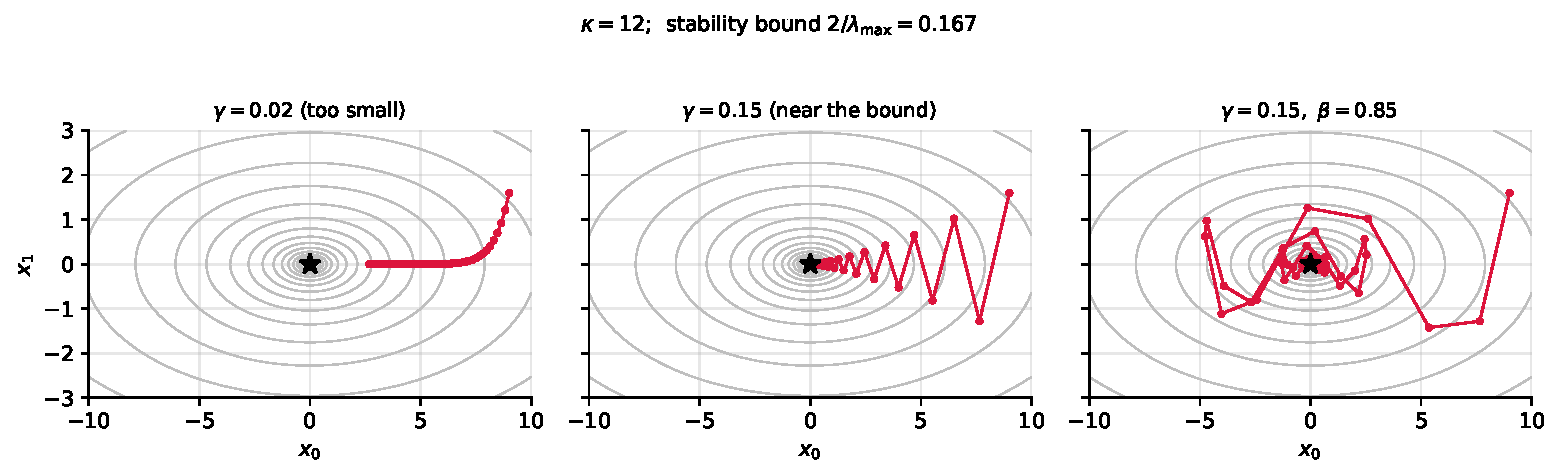
\includegraphics[width=0.98\textwidth]{BookFigures/chapter04_optimization/gd_paths_conditioning}
\caption{Gradient descent on a quadratic with $\kappa=12$.  Left: too small a step.  Centre: a step near the stability bound $2/\lambda_{\max}$, oscillating across the narrow direction.  Right: the same step with momentum $\beta=0.85$, which cancels the oscillation and accumulates along the flat direction.}
\label{fig:gdpaths}
\end{figure}


%----------------------------------------------------------------------
\section{Momentum}
\label{sec:momentum}

\index{momentum}
The first remedy is to give the iteration a memory of where it has been.
Momentum-based gradient descent replaces Eq.~(\ref{eq:4-gd}) by
\begin{equation}
  \bm{v}_{k+1} = \beta\bm{v}_k + \gamma\nabla C(\bm{\theta}_k),
  \qquad
  \bm{\theta}_{k+1} = \bm{\theta}_k - \bm{v}_{k+1},
  \label{eq:4-momentum}
\end{equation}
with $\beta\in[0,1)$ the \emph{momentum parameter}, typically $0.9$ (it plays
the same role as, and is deliberately given the same letter as, the $\beta_1$
of the Adam method in Section~\ref{sec:adam}).  The
update is no longer the current gradient but an exponentially weighted sum of
all gradients seen so far,
\begin{equation}
  \bm{v}_{k+1} = \gamma\sum_{j=0}^{k}\beta^{\,k-j}\nabla C(\bm{\theta}_j),
  \label{eq:4-momentumsum}
\end{equation}
with older gradients discounted geometrically.  Setting $\beta=0$ recovers
plain gradient descent.

\paragraph{Why it works.}
Return to the decoupled recursion~(\ref{eq:4-decoupled}).  Along an
eigendirection with eigenvalue $\lambda_i$, the gradient is
$\lambda_i\tilde{e}_i$ and the momentum iteration becomes a two-term
recurrence in $\tilde{e}$ rather than a one-term one.  Its behaviour splits
into two regimes, and the split is exactly what we want.

In a \emph{flat} direction, $\gamma\lambda_i\ll1$, successive gradients point
the same way and Eq.~(\ref{eq:4-momentumsum}) adds them up.  A constant
gradient $g$ accumulates to
\begin{equation}
  v_\infty = \gamma g \sum_{j=0}^{\infty}\beta^{\,j} = \frac{\gamma g}{1-\beta},
  \label{eq:4-momentumgain}
\end{equation}
so the effective step is multiplied by $1/(1-\beta)$ -- a factor of ten for
$\beta=0.9$.  The method accelerates precisely where plain gradient descent
crawls.

In a \emph{steep} direction, the iterate overshoots and the gradient reverses
sign at every step.  Successive terms in Eq.~(\ref{eq:4-momentumsum}) then
alternate in sign and largely cancel, so the accumulated step is
\emph{smaller} than the bare gradient.  The oscillation across the narrow
valley is damped.

Momentum thus amplifies the consistent and cancels the oscillatory, which is
the right treatment for the ill-conditioned landscape diagnosed in
Section~\ref{sec:learningrate}.  A careful analysis of the two-term recurrence
shows that with optimally chosen $\gamma$ and $\beta$ the contraction rate
improves from Eq.~(\ref{eq:4-gdrate}) to
\begin{equation}
  \frac{\sqrt{\kappa}-1}{\sqrt{\kappa}+1},
  \label{eq:4-momentumrate}
\end{equation}
so the iteration count scales with $\sqrt{\kappa}$ instead of $\kappa$.  For
$\kappa=10^{4}$ that is a hundredfold reduction.  The reader will notice that
$\sqrt{\kappa}$ is also the rate of the conjugate gradient method quoted in
Section~\ref{sec:cg}; this is not a coincidence, since both build their step
out of the current gradient and the previous direction.  Momentum is,
in effect, conjugate gradients with the optimal coefficients replaced by a
fixed constant that need not be recomputed and does not require the cost to be
quadratic.

\paragraph{A minimal example.}
The behaviour is easiest to see on $f(x)=x^{2}$, where the exact answer is
known.

Figure~\ref{fig:momentumrate} shows what the improvement from $\kappa$ to
$\sqrt{\kappa}$ is worth.  At $\kappa=10^{2}$ momentum saves an order of
magnitude in iterations; at $\kappa=10^{4}$, two.  Since
Eq.~(\ref{eq:4-kappasquared}) tells us that the least-squares Hessian has the
condition number of the design matrix \emph{squared}, condition numbers in
this range are entirely ordinary, and the saving is not academic.

\begin{figure}[htbp]
\centering
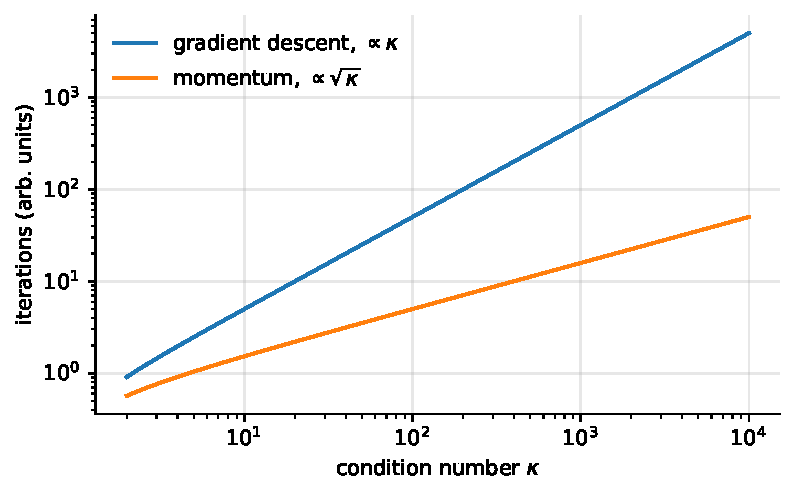
\includegraphics[width=0.62\textwidth]{BookFigures/chapter04_optimization/momentum_rate}
\caption{Iterations to fixed accuracy against the condition number, for gradient descent and for momentum with optimal parameters, from the rates (\ref{eq:4-gdrate}) and (\ref{eq:4-momentumrate}).}
\label{fig:momentumrate}
\end{figure}


\begin{Python}{}
import numpy as np

def objective(x):
    return x**2.0

def derivative(x):
    return 2.0 * x

def gradient_descent(derivative, bounds, n_iter, step_size, momentum=0.0,
                     rng=None):
    """Gradient descent with optional momentum, Eq. (4.momentum)."""
    rng = np.random.default_rng() if rng is None else rng
    solution = bounds[:, 0] + rng.random(len(bounds)) * (bounds[:, 1] - bounds[:, 0])
    change = 0.0
    solutions, scores = [], []
    for i in range(n_iter):
        gradient = derivative(solution)
        new_change = step_size * gradient + momentum * change
        solution = solution - new_change
        change = new_change
        solutions.append(solution.copy())
        scores.append(objective(solution))
    return solutions, scores


bounds = np.asarray([[-1.0, 1.0]])
rng = np.random.default_rng(4)
plain = gradient_descent(derivative, bounds, 30, 0.1, momentum=0.0,
                         rng=np.random.default_rng(4))
withmom = gradient_descent(derivative, bounds, 30, 0.1, momentum=0.3,
                           rng=np.random.default_rng(4))
print(f"after 30 steps: plain f = {plain[1][-1][0]:.3e}, "
      f"momentum f = {withmom[1][-1][0]:.3e}")
\end{Python}

For this one-dimensional problem $\kappa=1$ and there is nothing to fix, yet
momentum still helps by increasing the effective step through
Eq.~(\ref{eq:4-momentumgain}).  The dramatic gains appear when the eigenvalues
differ, which is the case for every realistic problem.

\begin{notebox}
\textbf{Machine learning connection.} A widely used variant is
\emph{Nesterov} momentum, which evaluates the gradient not at
$\bm{\theta}_k$ but at the point the momentum term is about to carry it to,
$\bm{\theta}_k-\beta\bm{v}_k$.  The intuition is that of looking ahead before
stepping: if the accumulated velocity is about to overshoot, the gradient at
the extrapolated point already points backwards and corrects the step early.
For convex problems this improves the constant in
Eq.~(\ref{eq:4-momentumrate}), and in deep learning frameworks it is usually
available as a flag on the standard momentum optimiser.
\end{notebox}

%----------------------------------------------------------------------
\section{Stochastic gradient descent}
\label{sec:sgd}

\index{stochastic gradient descent}\index{minibatch}\index{epoch}
The second remedy attacks a different problem: cost.

\paragraph{The idea.}
Almost every cost function in machine learning is a sum over data points,
\begin{equation}
  C(\bm{\theta}) = \sum_{i=1}^{n} c_i(\bm{x}_i,\bm{\theta}),
  \qquad
  \nabla_{\bm{\theta}}C(\bm{\theta})
   = \sum_{i=1}^{n}\nabla_{\bm{\theta}}c_i(\bm{x}_i,\bm{\theta}) .
  \label{eq:4-costsum}
\end{equation}
Computing the full gradient therefore costs one pass over the entire data set
for a single parameter update.  In large-scale applications -- the ImageNet
challenge has millions of training images -- this is extravagant: we spend an
enormous computation to obtain one number, most of whose precision is wasted,
since we are going to take another step immediately afterwards.

Stochasticity is introduced by evaluating the gradient on a random subset of
the data, called a \emph{minibatch}.  With $n$ data points and minibatches of
size $M$ there are $n/M$ minibatches, denoted $B_k$ with $k=1,\dots,n/M$.  If
$n=10$ and we choose five minibatches, each contains two points:
$B_1=(\bm{x}_1,\bm{x}_2)$ through $B_5=(\bm{x}_9,\bm{x}_{10})$.  Taking $M=n$
gives a single batch containing everything, which is ordinary gradient
descent; taking $M=1$ gives one point per batch.  We approximate
\begin{equation}
  \nabla_{\bm{\theta}}C(\bm{\theta})
   = \sum_{i=1}^{n}\nabla_{\bm{\theta}}c_i(\bm{x}_i,\bm{\theta})
   \;\longrightarrow\;
   \sum_{i\in B_k}\nabla_{\bm{\theta}}c_i(\bm{x}_i,\bm{\theta}),
  \label{eq:4-sgdgradient}
\end{equation}
and the update becomes
\begin{equation}
  \bm{\theta}_{j+1} = \bm{\theta}_j
    - \gamma_j\sum_{i\in B_k}\nabla_{\bm{\theta}}c_i(\bm{x}_i,\bm{\theta}),
  \label{eq:4-sgdupdate}
\end{equation}
with $k$ drawn at random with equal probability from $[1,n/M]$.  One pass
through all the minibatches is called an \emph{epoch}, and one typically
chooses a number of epochs and iterates over the minibatches within each.

Strictly, \emph{stochastic gradient descent} means using a single example at a
time, and the minibatch version should be called minibatch gradient descent;
but in practice everyone says SGD and means minibatches, and we shall do the
same.  Single-example updates are in fact rarely used, because vectorised
hardware evaluates a gradient on $100$ examples far faster than $100$
single-example gradients.  The minibatch size is a hyperparameter, but it is
seldom tuned by cross-validation: it is usually set by memory constraints, or
to a power of two such as $32$, $64$ or $128$, because vectorised operations
are fastest at those sizes.

\begin{Python}{}
import numpy as np

n = 100            # data points
M = 5              # size of each minibatch
m = int(n / M)     # number of minibatches
n_epochs = 10

for epoch in range(1, n_epochs + 1):
    for i in range(m):
        k = np.random.randint(m)     # pick the k-th minibatch at random
        # compute the gradient using the data in minibatch B_k
        # update theta with Eq. (4.sgdupdate)
        pass
\end{Python}

\paragraph{Two benefits.}
Taking the gradient on a subset has two distinct advantages.  It is
\emph{cheaper}: if $M\ll n$ the gradient costs a fraction of the full one, so
we take many more steps for the same computation.  And it introduces
\emph{noise}, which decreases the chance of the scheme becoming stuck in a
poor local minimum -- the deterministic objection raised in
Section~\ref{sec:graddescent}.  A stochastic iterate can be jostled out of a
shallow basin in a way a deterministic one cannot.

The corresponding disadvantages are that convergence is erratic rather than
monotone, that the iterate does not settle at the minimum but rattles around
in a neighbourhood whose size is set by the gradient noise and the learning
rate, and that the learning rate must be chosen with more care.

\paragraph{Speed against accuracy.}
It is worth being precise about the trade-off, because the folk statement that
``SGD converges faster'' conflates two different things.  Per \emph{iteration},
full-batch gradient descent makes more progress: it uses the exact gradient
and, for a strongly convex problem, converges geometrically at the rate of
Eq.~(\ref{eq:4-gdrate}).  Stochastic gradient descent, with a decaying
learning rate, converges at the far slower rate $\bigO(1/k)$ for strongly
convex problems and $\bigO(1/\sqrt{k})$ in general, because the gradient noise
does not vanish.  Per \emph{unit of computation}, however, SGD is
overwhelmingly ahead, since each of its iterations costs $M/n$ of a full one.
For a data set of a million points and a batch of a hundred, SGD performs ten
thousand updates in the time full-batch gradient descent performs one.

The memory picture is similarly stark: full-batch methods must hold the whole
data set, or at least stream it, for every update, whereas SGD needs only the
current minibatch.  This is what makes training on data sets larger than
memory possible at all, and it is the reason every deep learning framework is
built around minibatches.

By Section~\ref{sec:clt}, the noise in a minibatch gradient estimate falls as
$1/\sqrt{M}$: quadrupling the batch size halves the gradient noise at four
times the cost per step.  That unfavourable exchange rate is why very large
batches are not automatically better.

%......................................................................
\subsection{Learning rate schedules and stopping}
\label{sec:schedules}

\index{learning rate!schedule}
Because the gradient noise does not decay, a constant learning rate leaves the
iterate bouncing around the minimum forever.  The standard remedy is to let
$\gamma$ decay with time.  Let $e=0,1,2,\dots$ index the epoch, let $m$ be the
number of minibatches, and set $t=e\cdot m+i$ with $i=0,\dots,m-1$.  A common
choice is
\begin{equation}
  \gamma_j(t;t_0,t_1) = \frac{t_0}{t+t_1},
  \label{eq:4-timedecay}
\end{equation}
with $t_0,t_1>0$ fixed.  The learning rate starts at $t_0/t_1$ and decays
towards zero, so that the iterate eventually stops moving.  The classical
conditions for convergence, due to Robbins and Monro, are that
$\sum_t\gamma_t=\infty$ -- so that the iterate can still reach the minimum from
any starting point -- while $\sum_t\gamma_t^{2}<\infty$, so that the accumulated
noise is finite.  Equation~(\ref{eq:4-timedecay}) satisfies both.

\begin{Python}{}
import numpy as np

def step_length(t, t0, t1):
    return t0 / (t + t1)

n, M = 100, 5
m = int(n / M)
n_epochs, t0, t1 = 500, 1.0, 10.0

for epoch in range(1, n_epochs + 1):
    for i in range(m):
        k = np.random.randint(m)
        t = epoch * m + i
        gamma = step_length(t, t0, t1)
        # compute the minibatch gradient and update theta
print(f"gamma after {n_epochs} epochs: {step_length(n_epochs*m, t0, t1):g}")
\end{Python}

\paragraph{When do we stop?}
One possibility is to compute the full gradient every few epochs and stop when
its norm falls below a threshold.  But a vanishing gradient identifies a
stationary point, not necessarily a good one, so it is wiser to evaluate the
cost at that point, record it, and continue: if the criterion triggers again
later, keep whichever $\bm{\theta}$ gave the lower value.  Because the scheme
is random by design, repeating the whole computation gives a different answer
each time, and taking the best of several runs is a legitimate and common
strategy.

In machine learning the more useful criterion is not about the gradient at
all.  As advised in Section~\ref{sec:generalisation}, one monitors the cost on
a held-out validation set and stops when it begins to \emph{rise} while the
training cost is still falling.  This is \emph{early stopping}, and it is a
regularisation method as much as a termination rule: halting before the
variance term of Eq.~(\ref{eq:2-biasvariance}) has grown is another way of
trading a little bias for a lot of variance, in the same spirit as the Ridge
penalty of Section~\ref{sec:ridge}.

%=============================================================================
%  PART THREE: ADAPTIVE METHODS
%=============================================================================

\section{Why adapt the step size at all}
\label{sec:adaptive}

\index{adaptive learning rate}\index{second moment of the gradient}
In stochastic gradient descent, with or without momentum, we still have to
specify a schedule for the learning rate $\gamma_t$.  Section~\ref{sec:learningrate}
showed exactly why this is awkward, and it is worth restating the diagnosis in
the form that motivates what follows.

A fixed $\gamma$ is hard to get right.  If it is too large the updates overshoot
and the iteration oscillates or diverges, by Eq.~(\ref{eq:4-stability}); if it
is too small, convergence takes forever, by Eq.~(\ref{eq:4-gdrate}).  But the
deeper problem is not the choice of a number: it is that \emph{no single
number is right for all directions}.  The stability bound is set by
$\lambda_{\max}$ and the convergence rate by $\lambda_{\min}$, and when these
differ by orders of magnitude the step which is barely safe along the steep
direction is hopelessly small along the flat one.  Steep coordinates need
small steps; flat coordinates could take large ones.  In high-dimensional
problems with features of varying scale, or with sparse features that are
active only occasionally, the mismatch is severe.

Ideally our algorithm would keep track of curvature and take large steps in
shallow directions and small steps in steep ones.  That is precisely what
Newton's method~(\ref{eq:4-newtonopt}) does, by normalising the gradient with
$\bm{H}^{-1}$; and the invariance this buys is why
Section~\ref{sec:newton} called it the ideal.  The trouble, again, is the
$\bigO(p^{3})$ cost of forming and inverting the Hessian, which is out of the
question for large models.

The methods of this section are a compromise.  They approximate the curvature
information in $\bm{H}$ using only quantities already available -- the
gradients themselves -- and they restrict the approximation to a
\emph{diagonal} matrix, so that inverting it costs $\bigO(p)$ rather than
$\bigO(p^{3})$.  Instead of tracking the gradient alone, they track the
\emph{second moment} of the gradient.  The family includes AdaGrad, AdaDelta,
RMSProp and Adam, and we develop the three named in the chapter title.

\paragraph{The idea in one paragraph.}
Suppose we replace the scalar $\gamma$ by a diagonal matrix, so that coordinate
$j$ has its own step size $\gamma/\sqrt{r_j}$.  What should $r_j$ be?  Near a
minimum the gradient along direction $j$ behaves as $g_j\approx\lambda_j e_j$,
so a large curvature $\lambda_j$ produces large gradients and a small
curvature produces small ones.  \emph{The typical magnitude of the gradient in
a direction is a proxy for the curvature in that direction.}  Averaging
$g_j^{2}$ over recent steps therefore estimates something like $\lambda_j^{2}$
without ever forming a second derivative, and dividing by its square root
approximates the $\bm{H}^{-1/2}$ scaling.  This is the entire principle behind
AdaGrad, RMSProp and Adam; the three differ only in how the average is taken.

%----------------------------------------------------------------------
\section{AdaGrad}
\label{sec:adagrad}

\index{AdaGrad}
AdaGrad maintains a running sum of squared gradients for each coordinate.  Let
$\bm{g}_t=\nabla C_{i_t}(\bm{\theta}_t)$ be the gradient at step $t$, possibly
from a minibatch, and initialise $\bm{r}_0=\bm{0}$.  At each iteration
accumulate
\begin{equation}
  \bm{r}_t = \bm{r}_{t-1} + \bm{g}_t\circ\bm{g}_t,
  \label{eq:4-adagradaccum}
\end{equation}
where $\circ$ is the Hadamard product of Section~\ref{sec:vectors}, so that
$r_{t,j}=r_{t-1,j}+g_{t,j}^{2}$ for every coordinate $j$.  We may regard
$\bm{H}_t=\mathrm{diag}(\bm{r}_t)$ as a diagonal matrix of accumulated squared
gradients, with $\bm{H}_0=\bm{0}$.

The update scales the gradient by the inverse square root of this matrix,
\begin{equation}
  \bm{\theta}_{t+1} = \bm{\theta}_t - \gamma\,\bm{H}_t^{-1/2}\bm{g}_t,
  \label{eq:4-adagradmatrix}
\end{equation}
where $\bm{H}_t^{-1/2}$ is diagonal with entries $r_{t,j}^{-1/2}$.  In
coordinates each parameter has its own step size,
\begin{equation}
  \theta_{t+1,j} = \theta_{t,j} - \frac{\gamma}{\sqrt{r_{t,j}}}\,g_{t,j},
  \label{eq:4-adagradcoord}
\end{equation}
and in practice a small constant $\epsilon$ is added to the denominator for
numerical stability,
\begin{equation}
  \boxed{\;
  \theta_{t+1,j} = \theta_{t,j}
    - \frac{\gamma}{\sqrt{\epsilon + r_{t,j}}}\,g_{t,j} . \;}
  \label{eq:4-adagrad}
\end{equation}
The effective learning rate for parameter $j$ at time $t$ is
$\alpha_{t,j}=\gamma/\sqrt{\epsilon+r_{t,j}}$, which decreases as $r_{t,j}$
grows.

Note the resemblance between Eq.~(\ref{eq:4-adagradmatrix}) and Newton's
step~(\ref{eq:4-newtonopt}): both premultiply the gradient by an inverse
matrix built from curvature information.  AdaGrad differs in using
$\bm{H}^{-1/2}$ rather than $\bm{H}^{-1}$, in restricting $\bm{H}$ to be
diagonal, and in estimating it from gradient magnitudes rather than second
derivatives.

\paragraph{Properties.}
AdaGrad tunes the step size for each parameter automatically.  Parameters with
large or volatile gradients receive smaller steps; those with small or
infrequent gradients receive relatively larger ones.  No manual schedule is
needed: because $\bm{r}_t$ never decreases, the step sizes
$\gamma/\sqrt{r_{t,j}}$ are non-increasing, which has an effect similar to a
decaying learning rate but individualised per coordinate.

The benefit for sparse data is worth spelling out, since it is the setting for
which AdaGrad was designed.  Consider a rare feature -- a word appearing in
one document in a thousand.  Its gradient is zero on almost every minibatch,
so $r_{t,j}$ grows very slowly, so its learning rate stays high.  When the
feature finally does appear, the parameter takes a large, useful step instead
of the negligible one a global schedule would have permitted by then.
Frequently active features, conversely, accumulate large $r_{t,j}$ and their
learning rates fall automatically.

In convex optimisation AdaGrad achieves a convergence rate comparable to the
best fixed learning rate tuned in hindsight for the problem, which is a strong
guarantee and effectively removes the need to tune $\gamma$ by hand.

\paragraph{The limitation.}
Because $\bm{r}_t$ accumulates without bound, the learning rates decay
monotonically and can become vanishingly small long before the minimum is
reached.  On a convex problem this is tolerable, since the accumulated
gradients genuinely reflect the geometry.  In deep learning, where training
runs for many epochs and the landscape changes character as the iterate moves,
it is fatal: AdaGrad simply stops making progress.  The sum has an infinite
memory, and remembers gradients from a region of parameter space the iterate
left long ago.  RMSProp and Adam repair exactly this.

%----------------------------------------------------------------------
\section{RMSProp}
\label{sec:rmsprop}

\index{RMSProp}
RMSProp replaces the cumulative sum~(\ref{eq:4-adagradaccum}) by an
exponentially decaying average,
\begin{equation}
  \bm{v}_t = \rho\,\bm{v}_{t-1} + (1-\rho)\left(\nabla C(\bm{\theta}_t)\right)^{2},
  \label{eq:4-rmspropaccum}
\end{equation}
with the square taken element-wise and $\rho$ typically $0.9$ or $0.99$.  The
update is
\begin{equation}
  \boxed{\;
  \bm{\theta}_{t+1} = \bm{\theta}_t
    - \frac{\gamma}{\sqrt{\bm{v}_t+\epsilon}}\,\nabla C(\bm{\theta}_t) , \;}
  \label{eq:4-rmsprop}
\end{equation}
with the division element-wise.  The method was proposed by Geoffrey Hinton in
lecture notes in 2012 and never formally published, which has not prevented it
from becoming standard.

\paragraph{Why the change matters.}
Expanding Eq.~(\ref{eq:4-rmspropaccum}) shows what has happened,
\begin{equation}
  \bm{v}_t = (1-\rho)\sum_{j=0}^{t}\rho^{\,t-j}\bm{g}_j^{2},
  \label{eq:4-rmspropsum}
\end{equation}
which is a weighted average with weights summing to nearly one, rather than an
unbounded sum.  Gradients older than roughly $1/(1-\rho)$ steps -- ten steps
for $\rho=0.9$, a hundred for $\rho=0.99$ -- are effectively forgotten.  Two
consequences follow.  The quantity $\bm{v}_t$ is now an estimate of the
\emph{recent} mean square gradient, so it tracks the local curvature as the
iterate moves through a changing landscape.  And because it does not grow
without bound, the effective learning rate does not decay to zero: AdaGrad's
infinite memory problem is gone.

RMSProp is thus the same idea as AdaGrad with a finite memory, and the
resemblance to the momentum update~(\ref{eq:4-momentum}) is not accidental.
Both are exponential moving averages; momentum averages the gradient, RMSProp
averages its square.  It is natural to ask what happens if one does both.

%----------------------------------------------------------------------
\section{Adam}
\label{sec:adam}

\index{Adam optimizer}
Adam -- adaptive moment estimation -- was introduced by Kingma and Ba in
2014~\cite{kingma2014} and does exactly that.  It keeps running averages of
both the first and the second moment of the gradient and uses them to adapt
the learning rate for each parameter.  It is efficient for large problems
involving many data and many parameters, and it is the default optimiser in
most deep learning frameworks.

\paragraph{Why combine momentum and RMSProp?}
The two mechanisms address different defects and do not overlap.  Momentum
gives fast convergence by smoothing the gradient, accelerating along the
consistent long-term direction as in Eq.~(\ref{eq:4-momentumgain}) and damping
oscillations across narrow valleys.  RMSProp gives per-dimension scaling for
stability, handling features of different scales and sparse gradients.  Using
both means the direction of the step is chosen by an averaged gradient while
its length in each coordinate is chosen by the recent curvature estimate.

\paragraph{The two moments.}
Adam maintains, at each step $t$,
\begin{align}
  \bm{m}_t &= \beta_1\bm{m}_{t-1} + (1-\beta_1)\nabla C(\bm{\theta}_t)
   && \text{(first moment, the momentum term)},
  \label{eq:4-adamfirst}\\
  \bm{v}_t &= \beta_2\bm{v}_{t-1}
    + (1-\beta_2)\left(\nabla C(\bm{\theta}_t)\right)^{2}
   && \text{(second moment, the RMS term)},
  \label{eq:4-adamsecond}
\end{align}
with typical values $\beta_1=0.9$ and $\beta_2=0.999$, and
$\bm{m}_0=\bm{v}_0=\bm{0}$.

\paragraph{Bias correction.}
Those initialisations cause a problem which is worth deriving, because it
explains a step that otherwise looks arbitrary.  Suppose the gradient is
stationary with true second moment $\mathbb{E}[g^{2}]$.  Unrolling
Eq.~(\ref{eq:4-adamsecond}) as in Eq.~(\ref{eq:4-rmspropsum}) and taking the
expectation,
\begin{equation}
  \mathbb{E}[v_t] = (1-\beta_2)\sum_{j=1}^{t}\beta_2^{\,t-j}\,\mathbb{E}[g^{2}]
   = \mathbb{E}[g^{2}]\left(1-\beta_2^{\,t}\right),
  \label{eq:4-adambiasderiv}
\end{equation}
using the finite geometric sum.  The estimate is therefore too small by
exactly the factor $1-\beta_2^{t}$, and the same argument applies to
$\bm{m}_t$ with $\beta_1$.  The bias is severe at the start: with
$\beta_2=0.999$ the factor is $10^{-3}$ at $t=1$, so the raw $v_1$ underestimates
the true second moment by three orders of magnitude, and the step
$\gamma/\sqrt{v}$ would be enormous.  Dividing by the known factor removes the
bias exactly,
\begin{equation}
  \hat{\bm{m}}_t = \frac{\bm{m}_t}{1-\beta_1^{\,t}},
  \qquad
  \hat{\bm{v}}_t = \frac{\bm{v}_t}{1-\beta_2^{\,t}} .
  \label{eq:4-adambias}
\end{equation}
For small $t$ the correction is large, compensating for the initial zero; as
$t$ grows, $1-\beta_i^{t}\to1$ and the corrected moments converge to the raw
ones.  Bias correction is what makes Adam stable in its first iterations, and
it is the one ingredient AdaGrad and RMSProp lack.

\paragraph{The update.}
Finally,
\begin{equation}
  \boxed{\;
  \bm{\theta}_{t+1} = \bm{\theta}_t
    - \frac{\alpha}{\sqrt{\hat{\bm{v}}_t}+\epsilon}\,\hat{\bm{m}}_t , \;}
  \label{eq:4-adam}
\end{equation}
with $\epsilon$ a small constant, typically $10^{-8}$, preventing division by
zero.  Step by step: compute the gradient; update the two moving
averages~(\ref{eq:4-adamfirst}) and (\ref{eq:4-adamsecond}); bias-correct with
Eq.~(\ref{eq:4-adambias}); form the step
$\Delta\bm{\theta}_t=\hat{\bm{m}}_t/(\sqrt{\hat{\bm{v}}_t}+\epsilon)$; and
update the parameters.

\paragraph{Adam against its predecessors.}
AdaGrad uses per-coordinate scaling like Adam but has no momentum, and slows
down excessively because its accumulation never forgets.  RMSProp uses a
moving average of squared gradients, so it does not slow down, but includes
neither momentum nor bias correction.  Adam is, in effect, RMSProp plus
momentum plus bias correction: the first moment provides acceleration and
smoother convergence, the second moderates the step size per dimension, and
the correction ensures the estimates are sound from the first iteration.

\begin{notebox}
\textbf{Why these methods work: the summary argument.}  It is worth collecting
the thread that runs through Sections~\ref{sec:learningrate} to
\ref{sec:adam}, because each method is a response to the same diagnosis.

The trouble with gradient descent is the mismatch between one global step size
and a cost function whose curvature varies by direction; the iteration count
scales with $\kappa=\lambda_{\max}/\lambda_{\min}$ by
Eq.~(\ref{eq:4-gdrate}).  Newton's method removes the mismatch entirely by
premultiplying with $\bm{H}^{-1}$, but costs $\bigO(p^{3})$.

Momentum attacks the symptom: it cancels the oscillation along steep
directions and accumulates progress along flat ones, improving the rate from
$\kappa$ to $\sqrt{\kappa}$ at no extra cost.  It does not, however, use
different step sizes in different coordinates.

The adaptive methods attack the cause, by constructing a cheap diagonal
approximation to the curvature from the second moment of the gradient.  Where
gradients are persistently large the curvature is presumed large and the step
is shortened; where they are small the step is lengthened.  Dividing by
$\sqrt{v_j}$ is an $\bigO(p)$ stand-in for the $\bigO(p^{3})$ operation of
applying $\bm{H}^{-1/2}$.

Two observations follow.  The first is that these methods are approximately
invariant to the scaling of individual features, since multiplying a feature
by $c$ multiplies its gradient by $c$ and its accumulated second moment by
$c^{2}$, leaving the ratio unchanged.  That is why they are so much less
sensitive to preprocessing than plain gradient descent -- although, as
Section~\ref{sec:practicaltips} notes, standardising the inputs remains good
practice.  The second is that a diagonal approximation can only capture
curvature aligned with the coordinate axes.  A cost function whose narrow
valley runs diagonally in parameter space has a Hessian with large
off-diagonal entries, and no diagonal rescaling will fix it; this is the
residual gap between Adam and true second-order methods, and it is why
decorrelating the inputs helps even when the scales already match.
\end{notebox}

%----------------------------------------------------------------------
\section{Implementations}
\label{sec:adaptivecode}

The three algorithms are described in detail in Goodfellow, Bengio and
Courville~\cite{goodfellow2016}, chapter 8.  We give compact implementations
here, all applied to the same least-squares problem of
Section~\ref{sec:gdlinreg} so that they may be compared directly.

\begin{Python}{}
import numpy as np

def make_batches(n, batch_size, rng):
    """Shuffle the indices and split them into minibatches."""
    idx = rng.permutation(n)
    return [idx[i:i + batch_size] for i in range(0, n, batch_size)]


def sgd_adaptive(X, y, method="adam", n_epochs=100, batch_size=10,
                 gamma=0.01, beta=0.9, rho=0.99,
                 beta1=0.9, beta2=0.999, eps=1e-8, rng=None):
    """Stochastic gradient descent with the optimisers of this chapter.

    method is one of "plain", "momentum", "adagrad", "rmsprop", "adam".
    """
    rng = np.random.default_rng() if rng is None else rng
    n, p = X.shape
    theta = rng.normal(size=(p, 1))

    change = np.zeros((p, 1))          # momentum velocity, Eq. (4.momentum)
    r = np.zeros((p, 1))               # accumulated second moment
    m = np.zeros((p, 1))               # first moment, Eq. (4.adamfirst)
    t = 0

    for epoch in range(n_epochs):
        for batch in make_batches(n, batch_size, rng):
            t += 1
            Xb, yb = X[batch], y[batch]
            g = (2.0 / len(batch)) * Xb.T @ (Xb @ theta - yb)

            if method == "plain":
                update = gamma * g
            elif method == "momentum":
                change = gamma * g + beta * change
                update = change
            elif method == "adagrad":
                r += g * g                                   # Eq. (4.adagradaccum)
                update = gamma * g / (np.sqrt(r) + eps)        # Eq. (4.adagrad)
            elif method == "rmsprop":
                r = rho * r + (1 - rho) * g * g              # Eq. (4.rmspropaccum)
                update = gamma * g / (np.sqrt(r) + eps)        # Eq. (4.rmsprop)
            elif method == "adam":
                m = beta1 * m + (1 - beta1) * g              # Eq. (4.adamfirst)
                r = beta2 * r + (1 - beta2) * g * g          # Eq. (4.adamsecond)
                m_hat = m / (1 - beta1**t)                   # Eq. (4.adambias)
                r_hat = r / (1 - beta2**t)
                update = gamma * m_hat / (np.sqrt(r_hat) + eps)
            else:
                raise ValueError(f"unknown method {method}")

            theta -= update

    return theta
\end{Python}

Running all five on the data of Section~\ref{sec:gdlinreg} for a hundred
epochs with batches of ten, for three values of the learning rate, gives the
final cost values of Table~\ref{tab:optimcompare}.  The analytical solution of
Eq.~(\ref{eq:3-olssolution}) is $\hat{\bm{\theta}}=(4.030,2.806)$ with cost
$1.14947$, which is the floor.

\begin{table}[h]
\centering
\renewcommand{\arraystretch}{1.25}
\setlength{\tabcolsep}{12pt}
\begin{tabular}{lrrr}
\toprule
\textbf{Method} & $\gamma=0.01$ & $\gamma=0.1$ & $\gamma=0.5$\\
\midrule
Plain SGD          & $1.1499$  & $1.1532$ & $1.2274$\\
Momentum           & $1.1553$  & $1.5674$ & $1.3490$\\
AdaGrad            & $28.049$  & $1.2776$ & $\mathbf{1.1497}$\\
RMSProp            & $1.1516$  & $1.1512$ & $1.1904$\\
Adam               & $1.2185$  & $1.1514$ & $1.1565$\\
\bottomrule
\end{tabular}
\caption{Final value of the cost function~(\ref{eq:4-gdcost}) after $100$
epochs of stochastic gradient descent on the data of
Section~\ref{sec:gdlinreg}, for each optimiser and three learning rates.  The
analytical minimum is $1.14947$.  Note that no row is best at the same $\gamma$
as any other.}
\label{tab:optimcompare}
\end{table}

The table repays study, and not because it flatters the adaptive methods.

The first observation is that on this problem the sophisticated methods are
not better.  With $\gamma=0.01$ plain SGD reaches $1.1499$, within $0.04\%$ of
the optimum, while Adam manages only $1.2185$ and AdaGrad is catastrophic at
$28.05$ -- it has not arrived anywhere near the minimum.  This is exactly what
Section~\ref{sec:adagrad} predicted: the accumulated $\bm{r}_t$ drives the
effective step $\gamma/\sqrt{r_t}$ towards zero, and with $\gamma$ already small
the iterate stalls long before reaching the solution.  Nothing is wrong with
the implementation; the method is behaving as designed, and the design is
wrong for this problem.

The second observation explains the first.  Look along the rows rather than
down the columns.  AdaGrad is worst at $\gamma=0.01$ and \emph{best of all five}
at $\gamma=0.5$, where it essentially attains the analytical minimum.  Plain SGD
and momentum move the other way, degrading as $\gamma$ grows.  The reason is
that these methods do not use $\gamma$ to mean the same thing.  Plain gradient
descent multiplies $\gamma$ by the raw gradient, so the stability
bound~(\ref{eq:4-stability}) applies directly.  The adaptive methods divide by
$\sqrt{v_j}$ first, which renormalises the gradient to something of order
unity, so their $\gamma$ sets a step length in parameter space rather than a
multiple of the gradient.  \emph{A learning rate is not comparable across
optimisers}, and a comparison at a single fixed $\gamma$ -- which is what one
sees most often -- says more about which method happens to suit that number
than about the methods.

The third observation is the one to carry forward.  This problem has $p=2$,
is convex, and has a Hessian with eigenvalues $0.311$ and $3.728$, hence
$\kappa=11.97$ by Eq.~(\ref{eq:4-gdrate}).  That is a benign landscape, and
there is simply nothing for the adaptive machinery to repair; the overhead of
estimating curvature buys nothing because the curvature is already uniform.
The adaptive methods earn their place when $\kappa$ is large, when $p$ is
large, when the gradients are sparse, and when the cost is non-convex --
which is to say in the neural networks of the following chapters, and not
here.  Demonstrating a method on a problem it was not designed for is a good
way to understand what it actually does.

Figure~\ref{fig:optimisers} plots the same comparison as a function of the
epoch rather than as a final number, and it makes the second lesson of the
table unmistakable.  At $\gamma=0.01$ the adaptive methods are slower than plain
stochastic gradient descent and AdaGrad has effectively stopped; at $\gamma=0.5$
the ordering is reversed and AdaGrad is the best of the five.  Nothing about
the methods has changed between the panels.  Only the number $\gamma$ has, and it
means something different to each of them.

\begin{figure}[htbp]
\centering
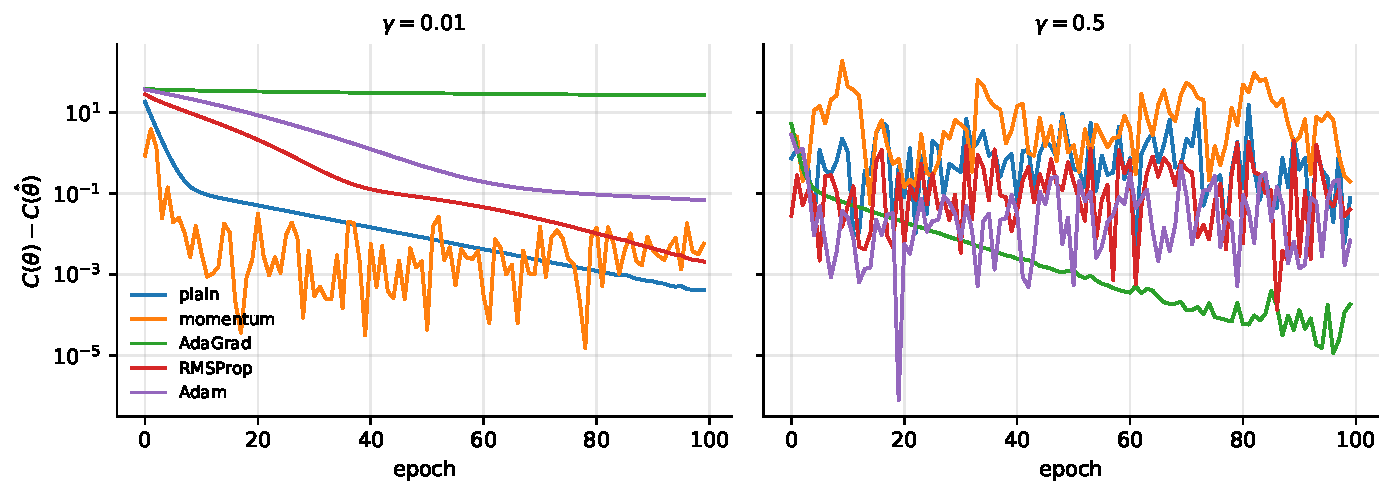
\includegraphics[width=0.95\textwidth]{BookFigures/chapter04_optimization/optimiser_comparison}
\caption{Excess cost against epoch for the five optimisers of Section~\ref{sec:adaptivecode} at two learning rates.  The vertical axis is $C(\bm{\theta})$ minus its value at the analytical minimum.  The ranking of the methods reverses between the panels.}
\label{fig:optimisers}
\end{figure}


\begin{notebox}
\textbf{Machine learning connection.} The default hyperparameters
$\beta_1=0.9$, $\beta_2=0.999$, $\epsilon=10^{-8}$ and $\alpha=10^{-3}$ from
the original paper are used almost universally and are usually a reasonable
starting point, which is a large part of Adam's popularity.  It should be
said, however, that adaptive methods do not always generalise as well as
plain SGD.  Several studies have found that models trained with Adam, RMSProp
or AdaGrad reach a worse test error than the same models trained with
well-tuned SGD with momentum, particularly in the overparameterised regime
where the number of parameters exceeds the number of data points.  Why this
should be so is not settled.  The practical advice is that Adam is an
excellent default for getting a model training at all, and that a carefully
tuned SGD with momentum is worth trying before the final result is reported.
\end{notebox}

%----------------------------------------------------------------------
\section{None of these can compete with Newton's method}
\label{sec:newtoncompete}

It is a useful corrective, having built up this machinery, to see how it fares
against Eq.~(\ref{eq:4-newtonopt}) on a problem where the Hessian is
affordable.  For the least-squares cost of Section~\ref{sec:gdlinreg} a single
Newton step lands on the exact minimum, by Eq.~(\ref{eq:4-newtonols}), while
the methods above need hundreds or thousands of iterations to get five decimal
places.

\begin{Python}{}
import numpy as np

# One Newton step solves the least-squares problem exactly
H = (2.0 / n) * X.T @ X
theta = rng.normal(size=(2, 1))
gradient = (2.0 / n) * X.T @ (X @ theta - y)
theta -= np.linalg.solve(H, gradient)
print("after one Newton step:", theta.ravel())
print("analytical solution:  ", (np.linalg.pinv(X.T @ X) @ X.T @ y).ravel())
\end{Python}

The two agree to machine precision.  The moral is not that we should use
Newton's method -- for a quadratic cost we would use the closed form of
Chapter~\ref{chap:lreg}, and for a large model we could not afford the
Hessian at all -- but that the gradient methods of this chapter are
\emph{approximations} to something better, adopted because of cost.  Every
improvement from momentum to Adam is a step back towards
Eq.~(\ref{eq:4-newtonopt}), recovering a little more curvature information for
a little more bookkeeping, and the quality of a method can fairly be judged by
how much of the Hessian it manages to imitate for $\bigO(p)$ work per step.

%=============================================================================
%  PART FOUR: TOOLS AND PRACTICE
%=============================================================================

\section{Automatic differentiation}
\label{sec:autodiff}

\index{automatic differentiation}
Every method in this chapter needs a gradient.  For linear regression we
computed it by hand in Eq.~(\ref{eq:4-gdgradient}); for a neural network with
a dozen layers, doing so by hand is possible but error-prone, and for a model
under active development it is impractical.  \emph{Automatic differentiation}
(AD), also called algorithmic differentiation, solves the problem completely,
and this section explains how.  We first say precisely what AD is not, then
derive its two modes from the chain rule, prove the one result about cost that
makes deep learning feasible, and finally show how the same ideas are used
from Python through the \texttt{JAX} library.

AD exploits the fact that every computer program, however complicated,
executes a sequence of elementary arithmetic operations and elementary
functions -- addition, multiplication, $\exp$, $\log$, $\sin$ -- each of whose
derivatives is known.  Applying the chain rule of Eq.~(\ref{eq:1-chainrule})
repeatedly to that sequence yields derivatives of arbitrary order,
\emph{accurate to working precision}, at a cost only a small constant factor
above that of the original program.  Both halves of that sentence -- the
accuracy and the cost -- are theorems, and we shall prove them.

%......................................................................
\subsection{Three ways to differentiate a program}
\label{sec:adthreeways}

\index{symbolic differentiation}\index{finite differences}
It is important to distinguish AD from the two things it is often confused
with.

\paragraph{Symbolic differentiation.}
A symbolic differentiator manipulates expressions: it takes the formula for $f$ and returns the formula
for $f'$.  This is what a computer-algebra system does and it is exact, but it
requires the program to be a single closed-form expression in the first place
-- no loops, no branches, no intermediate variables -- and it suffers from
\emph{expression swell}: the derivative of a product of $m$ factors has $m$
terms, the derivative of that has $m^{2}$, and the size of the formula grows
without any of the sharing of intermediate results that the original program
enjoyed.

\paragraph{Numerical differentiation.}
A numerical differentiator replaces the derivative by a difference quotient.  For a function of one
variable the central difference is
\begin{equation}
  f'(x) \approx D_h f(x) = \frac{f(x+h)-f(x-h)}{2h},
  \label{eq:4-centraldiff}
\end{equation}
and its error can be analysed exactly.  Expanding both terms in Taylor series
about $x$ and subtracting, all even powers of $h$ cancel and
\begin{equation}
  D_hf(x) = f'(x) + \frac{h^{2}}{6}f'''(x) + \bigO(h^{4}),
  \label{eq:4-truncation}
\end{equation}
the \emph{truncation error}, which shrinks as $h^{2}$.  This suggests taking
$h$ as small as possible.  But the two function values are computed in
floating point, each with a relative error of order the unit roundoff
$\epsilon_M\approx2.2\times10^{-16}$ of Section~\ref{sec:norms}, so the
numerator carries an absolute error of order $\epsilon_M|f(x)|$ and the
quotient an error of order $\epsilon_M|f(x)|/h$: the \emph{rounding error},
which \emph{grows} as $h$ shrinks.  This is catastrophic cancellation, the
subtraction of two nearly equal numbers.  The total error is therefore of the
form
\begin{equation}
  E(h) \approx \frac{h^{2}}{6}\left|f'''(x)\right|
             + \frac{\epsilon_M\left|f(x)\right|}{h},
  \label{eq:4-fderror}
\end{equation}
and setting $dE/dh=0$ gives the optimal step and the best attainable accuracy,
\begin{equation}
  h^{*} = \left(\frac{3\epsilon_M|f|}{|f'''|}\right)^{1/3}
        \sim \epsilon_M^{1/3}\approx 6\times10^{-6},
  \qquad
  E(h^{*}) \sim \epsilon_M^{2/3}\approx 4\times10^{-11}.
  \label{eq:4-fdoptimal}
\end{equation}
A central difference can never deliver more than about two thirds of the
available digits, and only if $h$ is chosen well; the one-sided difference
$(f(x+h)-f(x))/h$ has truncation error $\bigO(h)$ and does correspondingly
worse, $E\sim\epsilon_M^{1/2}\approx10^{-8}$.  Figure~\ref{fig:4-fdvsad}
shows the curve~(\ref{eq:4-fderror}) measured for a concrete function.  And
the cost is the second objection: for a function of $p$ variables the gradient
needs $2p$ evaluations, or $p+1$ for one-sided differences, and for $p=10^{7}$
that is a week of computing to obtain one, mediocre, gradient.

\paragraph{Automatic differentiation.}
AD has neither defect.  It computes the numerical value of the derivative at a
point, not a formula, so there is no expression swell; it does so by
propagating exact derivative rules through the program, so there is no
truncation error and no step $h$ to choose; and, in the mode used for
training, it obtains all $p$ components of the gradient for the price of a
small constant number of evaluations of $f$.  Reverse-mode AD is what
backpropagation is.  For $p=10^{7}$ the difference against finite differences
is between a fraction of a second and a week, and it is the reason the models
of the later chapters can be trained at all.

%......................................................................
\subsection{Evaluation traces and the computational graph}
\label{sec:adtrace}

\index{computational graph}\index{evaluation trace}
The object AD works on is not the formula for $f$ but the sequence of
operations a program executes to evaluate it.  Consider the function
\begin{equation}
  f(x_1,x_2) = \ln x_1 + x_1x_2 - \sin x_2 ,
  \label{eq:4-adexample}
\end{equation}
which a program evaluates as the following list of assignments, each applying
one elementary operation $\varphi_i$ to variables already computed:
\begin{equation}
  \begin{aligned}
    v_{-1} &= x_1, & v_0 &= x_2, \\
    v_1 &= \ln v_{-1}, & v_2 &= v_{-1}\,v_0, & v_3 &= \sin v_0, \\
    v_4 &= v_1 + v_2, & v_5 &= v_4 - v_3, & y &= v_5 .
  \end{aligned}
  \label{eq:4-adtrace}
\end{equation}
This is the \emph{evaluation trace}, or Wengert list, of $f$
\cite{wengert1964,griewank2008}: the inputs are numbered $v_{1-n},\dots,v_0$,
the intermediate results $v_1,\dots,v_\ell$ in the order in which they are
computed, and the output is the last of them.  Drawn as a directed graph with
an edge $j\to i$ whenever $v_i$ depends directly on $v_j$, it is the
\emph{computational graph} of Fig.~\ref{fig:4-compgraph}.  Any program made
of elementary operations has such a trace -- loops unroll into repeated
assignments, and a branch simply selects which assignments are executed for
the given input -- and that is what makes AD applicable to programs rather
than to formulae.  A neural network is a particularly regular trace: the
matrix products, additions and activation functions of Chapter~\ref{chap:nn},
one layer after another.

\begin{figure}[htbp]
\centering
\begin{tikzpicture}[>=Latex,x=1cm,y=1cm,
  inp/.style={circle,draw=black!65,fill=Blue3!12,minimum size=8.5mm,
              inner sep=0pt,font=\small},
  op/.style={circle,draw=black!65,fill=black!5,minimum size=8.5mm,
             inner sep=0pt,font=\small},
  outp/.style={circle,draw=black!65,fill=Red3!12,minimum size=8.5mm,
               inner sep=0pt,font=\small},
  lab/.style={font=\footnotesize,black!60}]
  \node[inp] (x1) at (0, 1.6) {$v_{-1}$};
  \node[inp] (x2) at (0,-1.6) {$v_{0}$};
  \node[op]  (v1) at (2.4, 2.4) {$v_1$};
  \node[op]  (v2) at (2.4, 0.0) {$v_2$};
  \node[op]  (v3) at (2.4,-2.4) {$v_3$};
  \node[op]  (v4) at (4.8, 1.2) {$v_4$};
  \node[outp](v5) at (7.2, 0.0) {$v_5$};
  \draw[->,black!70] (x1) -- (v1);
  \draw[->,black!70] (x1) -- (v2);
  \draw[->,black!70] (x2) -- (v2);
  \draw[->,black!70] (x2) -- (v3);
  \draw[->,black!70] (v1) -- (v4);
  \draw[->,black!70] (v2) -- (v4);
  \draw[->,black!70] (v4) -- (v5);
  \draw[->,black!70] (v3) -- (v5);
  \draw[->,black!70] (v5) -- ++(1.4,0) node[right,font=\small] {$y$};
  \node[lab] at (0, 2.6) {$x_1$};
  \node[lab] at (0,-2.6) {$x_2$};
  \node[lab] at (2.4, 3.2) {$\ln$};
  \node[lab] at (2.4, 0.8) {$\times$};
  \node[lab] at (2.4,-3.2) {$\sin$};
  \node[lab] at (4.8, 2.0) {$+$};
  \node[lab] at (7.2, 0.8) {$-$};
  \node[lab] at (-0.2,-3.4) {inputs};
  \node[lab] at (7.2,-3.4) {output};
\end{tikzpicture}
\caption{The computational graph of the evaluation trace~(\ref{eq:4-adtrace})
for $f(x_1,x_2)=\ln x_1+x_1x_2-\sin x_2$.  Each node is one elementary
operation applied to its predecessors.  Forward-mode AD sweeps this graph from
left to right, carrying a derivative $\dot v_i$ with every value; reverse-mode
AD first evaluates the values from left to right and then sweeps back from
right to left, carrying an adjoint $\bar v_i=\partial y/\partial v_i$ with
every node.}
\label{fig:4-compgraph}
\end{figure}

For each node the derivative of the elementary operation with respect to each
of its arguments -- its \emph{local} or \emph{partial} derivative -- is known
in closed form:
\begin{equation}
  \frac{\partial v_1}{\partial v_{-1}} = \frac{1}{v_{-1}},\quad
  \frac{\partial v_2}{\partial v_{-1}} = v_0,\quad
  \frac{\partial v_2}{\partial v_{0}} = v_{-1},\quad
  \frac{\partial v_3}{\partial v_{0}} = \cos v_0,\quad
  \frac{\partial v_4}{\partial v_{1}} = \frac{\partial v_4}{\partial v_{2}} = 1,\quad
  \frac{\partial v_5}{\partial v_{4}} = 1,\quad
  \frac{\partial v_5}{\partial v_{3}} = -1 .
  \label{eq:4-adlocal}
\end{equation}
Everything AD does is to combine these local derivatives by the chain rule.
The only question is in which order, and there are two natural answers.

%......................................................................
\subsection{Forward mode: tangents and dual numbers}
\label{sec:adforward}

\index{forward-mode differentiation}\index{dual numbers}
Fix a direction $\dot{\bm{x}}\in\mathbb{R}^{n}$ in the input space and define
for every node its \emph{tangent}, the directional derivative
\begin{equation}
  \dot v_i = \sum_{k=1}^{n}\frac{\partial v_i}{\partial x_k}\,\dot x_k
           = \frac{d}{d\epsilon}\,v_i(\bm{x}+\epsilon\dot{\bm{x}})\Big|_{\epsilon=0}.
  \label{eq:4-tangentdef}
\end{equation}
Since $v_i=\varphi_i(v_j:j\prec i)$ depends only on its predecessors, the
chain rule gives the \emph{forward recursion}
\begin{equation}
  \dot v_i = \sum_{j\prec i}\frac{\partial\varphi_i}{\partial v_j}\,\dot v_j ,
  \qquad i=1,\dots,\ell,
  \label{eq:4-forwardrec}
\end{equation}
started from $\dot v_{1-n},\dots,\dot v_0$ set equal to the chosen direction
$\dot x_1,\dots,\dot x_n$.  The recursion runs in the same order as the
evaluation itself, so each tangent can be computed alongside its value, and
when the sweep reaches the output it holds $\dot y=\nabla f(\bm{x})^{T}\dot{\bm{x}}$.
For our example with $\dot{\bm{x}}=(1,0)$, that is $\partial f/\partial x_1$,
the sweep at $(x_1,x_2)=(2,5)$ reads
\begin{equation}
  \begin{aligned}
    \dot v_{-1} &= 1, & \dot v_0 &= 0,\\
    \dot v_1 &= \dot v_{-1}/v_{-1} = 0.5, &
    \dot v_2 &= \dot v_{-1}v_0 + v_{-1}\dot v_0 = 5, &
    \dot v_3 &= \cos(v_0)\,\dot v_0 = 0,\\
    \dot v_4 &= \dot v_1+\dot v_2 = 5.5, &
    \dot v_5 &= \dot v_4-\dot v_3 = 5.5 ,
  \end{aligned}
  \label{eq:4-forwardsweep}
\end{equation}
and indeed $\partial f/\partial x_1 = 1/x_1 + x_2 = 5.5$.  To obtain
$\partial f/\partial x_2$ the whole sweep is repeated with
$\dot{\bm{x}}=(0,1)$.

\paragraph{Dual numbers.}
There is an elegant algebraic way to say the same thing.  Introduce a symbol
$\varepsilon$ with $\varepsilon^{2}=0$ (but $\varepsilon\neq0$) and consider
\emph{dual numbers} $a+b\varepsilon$ with $a,b\in\mathbb{R}$.  They add
componentwise and multiply as
\begin{equation}
  (a+b\varepsilon)(c+d\varepsilon) = ac + (ad+bc)\varepsilon ,
  \label{eq:4-dualmult}
\end{equation}
because the $\varepsilon^{2}$ term vanishes.  Now let $g$ be any function with
a Taylor series and evaluate it at a dual argument.  Every power of
$\varepsilon$ beyond the first is zero, so the series terminates:
\begin{equation}
  g(a+b\varepsilon) = g(a) + g'(a)\,b\varepsilon
     + \tfrac{1}{2}g''(a)\,b^{2}\varepsilon^{2}+\dots
     = g(a) + g'(a)\,b\varepsilon .
  \label{eq:4-dualtaylor}
\end{equation}
The dual part is exactly the tangent~(\ref{eq:4-forwardrec}) of $g$: dual
numbers carry a value and a derivative together, and the multiplication
rule~(\ref{eq:4-dualmult}) \emph{is} the product rule.  Applying $g$ to
$x+1\cdot\varepsilon$ and reading off the coefficient of $\varepsilon$
therefore returns $g'(x)$ exactly -- not approximately, since nothing was
truncated: the series terminates by the algebra of $\varepsilon$, not by
neglecting small terms.  This is forward-mode AD in one line, and it can be
implemented in a few more.  The following class overloads the arithmetic
operators of Python so that ordinary code, written with no thought of
derivatives, computes them when handed a dual argument.

\begin{Python}{}
import math

class Dual:
    """A dual number a + b*eps with eps**2 = 0: a value and its derivative."""
    def __init__(self, val, dot=0.0):
        self.val, self.dot = val, dot
    def _lift(o):                       # promote plain floats to duals
        return o if isinstance(o, Dual) else Dual(o)
    def __add__(self, o):
        o = Dual._lift(o); return Dual(self.val + o.val, self.dot + o.dot)
    __radd__ = __add__
    def __sub__(self, o):
        o = Dual._lift(o); return Dual(self.val - o.val, self.dot - o.dot)
    def __mul__(self, o):               # the product rule, Eq. (4.dualmult)
        o = Dual._lift(o)
        return Dual(self.val * o.val, self.val * o.dot + self.dot * o.val)
    __rmul__ = __mul__
    def __truediv__(self, o):           # the quotient rule
        o = Dual._lift(o)
        return Dual(self.val / o.val,
                    (self.dot * o.val - self.val * o.dot) / o.val**2)
    def __pow__(self, k):
        return Dual(self.val**k, k * self.val**(k - 1) * self.dot)

# elementary functions: value and local derivative, Eq. (4.dualtaylor)
def sin(d): return Dual(math.sin(d.val), math.cos(d.val) * d.dot)
def exp(d): return Dual(math.exp(d.val), math.exp(d.val) * d.dot)
def log(d): return Dual(math.log(d.val), d.dot / d.val)

def f(x1, x2):                          # Eq. (4.adexample), ordinary code
    return log(x1) + x1 * x2 - sin(x2)

# seed the tangent of the variable we differentiate with respect to
print("df/dx1 =", f(Dual(2.0, 1.0), Dual(5.0, 0.0)).dot)   # 1/x1 + x2 = 5.5
print("df/dx2 =", f(Dual(2.0, 0.0), Dual(5.0, 1.0)).dot)   # x1 - cos(x2)
print("exact  =", 0.5 + 5.0, 2.0 - math.cos(5.0))
\end{Python}

\paragraph{Jacobian--vector products and the cost of forward mode.}
For a vector-valued $\bm{f}:\mathbb{R}^{n}\to\mathbb{R}^{m}$ with Jacobian
$\bm{J}\in\mathbb{R}^{m\times n}$ as in Eq.~(\ref{eq:1-jacobian}), one forward
sweep with seed $\dot{\bm{x}}$ returns
\begin{equation}
  \dot{\bm{y}} = \bm{J}\,\dot{\bm{x}} ,
  \label{eq:4-jvp}
\end{equation}
a \emph{Jacobian--vector product} (JVP), without ever forming $\bm{J}$.
Seeding with the unit vector $\bm{e}_k$ returns the $k$-th column of the
Jacobian, so the full Jacobian costs $n$ sweeps and the gradient of a scalar
function of $p$ parameters costs $p$ sweeps -- the same count as finite
differences, only exact.  Each sweep costs a small multiple of one function
evaluation, since Eq.~(\ref{eq:4-forwardrec}) adds to each elementary
operation a bounded number of further ones.  Forward mode is therefore the
right tool when the number of \emph{inputs} is small: the sensitivity of a
whole network output to one physical parameter, or the derivatives with
respect to one or two spatial coordinates that Chapter~\ref{chap:nnde} needs
when a network is made to satisfy a differential equation.  It is the wrong
tool for training, where $p$ is enormous and the output is a single scalar.

%......................................................................
\subsection{Reverse mode: adjoints}
\label{sec:adreverse}

\index{reverse-mode differentiation}\index{adjoint}\index{backpropagation}
Reverse mode fixes the \emph{output} instead of the input.  For a scalar
output $y$ define the \emph{adjoint} of every node,
\begin{equation}
  \bar v_i = \frac{\partial y}{\partial v_i},
  \label{eq:4-adjointdef}
\end{equation}
the sensitivity of the final result to that intermediate value.  Since $y$
depends on $v_j$ only through the nodes $v_i$ that consume it, the chain rule
gives the \emph{reverse recursion}
\begin{equation}
  \bar v_j = \sum_{i\succ j}\bar v_i\,\frac{\partial\varphi_i}{\partial v_j},
  \qquad j=\ell-1,\dots,1-n,
  \label{eq:4-reverserec}
\end{equation}
started from $\bar v_\ell=\partial y/\partial y=1$.  Compare this with the
forward recursion~(\ref{eq:4-forwardrec}): the same local derivatives appear,
but the sum now runs over the \emph{successors} of a node and the recursion
runs \emph{backwards} through the trace, from output to inputs.  When it
reaches the inputs it holds $\bar v_{1-n},\dots,\bar v_0$, which is the whole
gradient $\nabla f(\bm{x})$ -- all $n$ components from a single sweep.  For
our example, with the values from the forward evaluation at $(2,5)$,
\begin{equation}
  \begin{aligned}
    \bar v_5 &= 1,\\
    \bar v_4 &= \bar v_5\cdot1 = 1, &
    \bar v_3 &= \bar v_5\cdot(-1) = -1,\\
    \bar v_1 &= \bar v_4\cdot1 = 1, &
    \bar v_2 &= \bar v_4\cdot1 = 1,\\
    \bar v_0 &= \bar v_3\cos v_0 + \bar v_2 v_{-1} = 2-\cos5 = 1.716, &
    \bar v_{-1} &= \bar v_2 v_0 + \bar v_1/v_{-1} = 5 + 0.5 = 5.5 ,
  \end{aligned}
  \label{eq:4-reversesweep}
\end{equation}
which are $\partial f/\partial x_2$ and $\partial f/\partial x_1$, both
obtained at once.  The two contributions to $\bar v_0$ are the two paths
from $v_0$ to $y$ in Fig.~\ref{fig:4-compgraph}: the chain rule sums over
paths, and the reverse sweep organises that sum so that each edge is visited
once.

Reverse mode has a price that forward mode does not: the local derivatives
in Eq.~(\ref{eq:4-reverserec}) depend on the values $v_j$ -- $\cos v_0$,
$v_{-1}$, $1/v_{-1}$ above -- and those must be available when the backward
sweep needs them, in the reverse of the order in which they were produced.
The forward evaluation must therefore be recorded, on what is called the
\emph{tape}, and the memory cost of reverse mode is proportional to the length
of the trace rather than to the number of variables.  This is why training a
deep network is memory-bound: every activation of every layer is stored until
the backward pass has consumed it.

\paragraph{Vector--Jacobian products.}
For a vector-valued function seeded with a covector $\bar{\bm{y}}\in\mathbb{R}^{m}$
the reverse sweep returns
\begin{equation}
  \bar{\bm{x}}^{T} = \bar{\bm{y}}^{T}\bm{J},
  \qquad\text{equivalently}\qquad
  \bar{\bm{x}} = \bm{J}^{T}\bar{\bm{y}} ,
  \label{eq:4-vjp}
\end{equation}
a \emph{vector--Jacobian product} (VJP): one row of $\bm{J}$ per sweep, and
the full Jacobian in $m$ sweeps.  Equation~(\ref{eq:4-vjp}) is precisely
Eq.~(\ref{eq:1-chainrule}), a gradient propagated backwards by multiplication
with a transposed Jacobian, and it is why backpropagation was described in
Section~\ref{sec:chainrule} as the chain rule with the products taken in the
cheapest order.

\paragraph{The cheap gradient principle.}
The result that makes all of deep learning possible is the following.

\begin{proposition}[Cheap gradient principle]
\label{prop:4-cheapgradient}
Let $f:\mathbb{R}^{p}\to\mathbb{R}$ be evaluated by a trace of $\ell$
elementary operations, each of which has at most two arguments and whose
local derivatives cost at most a fixed multiple of the operation itself.
Then reverse-mode AD computes $f(\bm{x})$ and the complete gradient
$\nabla f(\bm{x})$ with at most $c\,\ell$ operations, where $c\le4$ is a
constant \emph{independent of $p$}.
\end{proposition}

\begin{proof}
The forward evaluation costs $\ell$ operations and records the trace.  In the
reverse recursion~(\ref{eq:4-reverserec}) each edge $j\to i$ of the graph
contributes exactly one term $\bar v_i\,\partial\varphi_i/\partial v_j$: one
multiplication, one addition into $\bar v_j$, and the evaluation of the local
derivative, which by hypothesis costs a bounded amount and often nothing at
all (for $+$ it is $1$, for $\times$ it is the other argument, already on the
tape).  Since each node has at most two incoming edges, the number of edges is
at most $2\ell$ and the reverse sweep costs at most a fixed multiple of $2\ell$
operations.  Adding the forward evaluation gives the bound, and nowhere did
$p$ enter: it determines how many adjoints are \emph{read off} at the end,
not how many operations are performed.
\end{proof}

The result is due to Baur and Strassen~\cite{baur1983} in the setting of
arithmetic circuits and to Linnainmaa~\cite{linnainmaa1976} and, independently,
the backpropagation literature in the setting of programs; the survey by
Baydin et al.~\cite{baydin2018} traces the history.  In practice the constant
is nearer $2$--$3$ than $4$: a gradient costs about as much as two or three
function evaluations.  Set against the $p+1$ evaluations of finite
differences or the $p$ sweeps of forward mode, this is the entire difference
between what can and cannot be trained.

\begin{notebox}
\textbf{Machine learning connection.}
Backpropagation, the algorithm of Chapter~\ref{chap:nn} that trains every
neural network, is Eq.~(\ref{eq:4-reverserec}) specialised to the layered
trace of a network.  The forward pass computes and stores the activations;
the backward pass propagates the adjoint of the cost -- the ``error'' of the
older literature -- from the output layer to the input, one transposed
weight matrix at a time, exactly as in Eq.~(\ref{eq:4-vjp}).  Nothing in
backpropagation is specific to networks: it is reverse-mode AD, and modern
frameworks make no distinction.
\end{notebox}

%......................................................................
\subsection{Forward or reverse: the chain rule as a matrix product}
\label{sec:adorder}

\index{chain rule!matrix form}
The cleanest way to see why the two modes differ in cost is to write a program
as a composition of $L$ stages,
$\bm{f}=\bm{f}_L\circ\bm{f}_{L-1}\circ\cdots\circ\bm{f}_1$, with
$\bm{f}_k:\mathbb{R}^{n_{k-1}}\to\mathbb{R}^{n_k}$, $n_0=n$ and $n_L=m$.  The
chain rule of Eq.~(\ref{eq:1-chainrulerow}) says that the Jacobian is a
product of the stage Jacobians,
\begin{equation}
  \bm{J} = \bm{J}_L\,\bm{J}_{L-1}\cdots\bm{J}_1 ,
  \qquad
  \bm{J}_k = \frac{\partial\bm{f}_k}{\partial\bm{x}_{k-1}}\in\mathbb{R}^{n_k\times n_{k-1}} .
  \label{eq:4-jacobianchain}
\end{equation}
Matrix multiplication is associative, so this product may be evaluated in any
order, and the orders differ enormously in cost.  Forward mode multiplies from
the right, $\bm{J}\dot{\bm{x}}=\bm{J}_L(\cdots(\bm{J}_2(\bm{J}_1\dot{\bm{x}})))$,
so every intermediate is a vector of length $n_k$ and never a matrix.  Reverse
mode multiplies from the left, $\bar{\bm{y}}^{T}\bm{J}
=(((\bar{\bm{y}}^{T}\bm{J}_L)\bm{J}_{L-1})\cdots)\bm{J}_1$, and again every
intermediate is a vector.  If the stage Jacobians are dense the cost of the
right-to-left product is $\sum_k n_kn_{k-1}$ per column, hence
$n\sum_kn_kn_{k-1}$ for the whole Jacobian, while the left-to-right product
costs $m\sum_kn_kn_{k-1}$.  The rule is therefore simple: use forward mode
when $n\ll m$ and reverse mode when $m\ll n$.  Training a model is the
extreme case $m=1$, $n=p$, and reverse mode wins by a factor $p$.  When $n$
and $m$ are comparable, neither mode is optimal and finding the cheapest
bracketing of Eq.~(\ref{eq:4-jacobianchain}) -- the optimal Jacobian
accumulation problem -- is NP-hard, though good heuristics exist
\cite{griewank2008}.

\paragraph{Second derivatives.}
The two modes compose, and their composition gives cheap access to curvature.
The Hessian of a scalar $f$ is the Jacobian of its gradient, and the
Hessian--vector product is a directional derivative of the gradient,
\begin{equation}
  \bm{H}\bm{v}
   = \frac{d}{d\epsilon}\nabla f(\bm{x}+\epsilon\bm{v})\Big|_{\epsilon=0} .
  \label{eq:4-hvp}
\end{equation}
The right-hand side is a forward-mode derivative, in the direction $\bm{v}$,
of a function -- the gradient -- that is itself computed by reverse mode.
This \emph{forward-over-reverse} construction costs a small constant times
one gradient, hence a small constant times one function evaluation, and it
never forms the $p\times p$ Hessian.  That is exactly the price at which
Section~\ref{sec:newtoncompete} said curvature information could \emph{not}
be had; the truncated-Newton and conjugate-gradient methods of the
optimisation literature~\cite{nocedal2006} use Eq.~(\ref{eq:4-hvp}) to run
Newton's method~(\ref{eq:4-newtonopt}) with only Hessian--vector products,
and the natural-gradient methods of Chapter~\ref{chap:nn} rely on the same
device.  The full Hessian, when it is wanted, is $p$ such products,
$\bm{H}=\bm{H}[\bm{e}_1,\dots,\bm{e}_p]$, and this is how
\texttt{jax.hessian} computes it.

%......................................................................
\subsection{Accuracy, and points where the derivative does not exist}
\label{sec:adaccuracy}

We claimed that AD is accurate to working precision, and the claim can now be
made precise.  The recursions~(\ref{eq:4-forwardrec}) and
(\ref{eq:4-reverserec}) are exact identities; the only errors are the rounding
errors of the floating-point operations that implement them.  Each tangent or
adjoint is obtained from its predecessors by a short chain of multiplications
and additions of quantities that were themselves computed to relative accuracy
$\bigO(\epsilon_M)$, so the derivative inherits the numerical stability of the
function evaluation itself: if the program computes $f$ to $d$ correct digits
it computes $\nabla f$ to about $d$ correct digits as well.  There is no
step $h$, no cancellation of nearly equal numbers, and no term of the form
$\epsilon_M/h$.  In Fig.~\ref{fig:4-fdvsad} the AD derivative sits at the
floor of the plot, at $10^{-16}$, for the same reason that the function value
does.

The one genuine limitation is that AD differentiates the program actually
executed.  At a point where the function is not differentiable -- $|x|$ at
zero, or the ReLU activation $\max(0,x)$ of Chapter~\ref{chap:nn} at $x=0$ --
the program takes one of the two branches and AD returns the derivative of
that branch, typically $0$ or $1$ by convention.  This is a valid
\emph{subgradient} and is harmless in practice, since the set of such points
has measure zero and an iterate never lands on it exactly.  More insidious is
a program that computes a smooth function by a non-smooth route, for instance
$\sqrt{x^{2}}$ for $|x|$ or a table lookup with interpolation, whose AD
derivative is that of the route rather than of the function.  Writing
functions with AD in mind -- using the library's own $\log(1+e^{x})$,
$\log\sum\exp$ and similar numerically careful primitives, whose derivative
rules are hand-written -- avoids both this and overflow in intermediate
values.

%......................................................................
\subsection{Automatic differentiation in Python: autograd and JAX}
\label{sec:adpython}

\index{JAX}\index{autograd}
Two libraries deliver the machinery above to ordinary numpy code.  The older
\texttt{autograd} package overloads the numpy functions with dual-number-like
objects that record a tape, exactly as the \texttt{Dual} class above did for
the standard library, and it remains a good way to see the mechanism at work:

\begin{Python}{}
import autograd.numpy as np
from autograd import grad

def f(x):
    return np.sin(2 * np.pi * x + x**2)

df = grad(f)                 # df is a Python function, the derivative of f
print(df(1.0))               # (2 pi + 2) cos(2 pi + 1) = 4.475424121402227

# It composes: the second derivative is just grad applied twice
d2f = grad(grad(f))
print(d2f(1.0))
\end{Python}

For current work we recommend \emph{JAX}~\cite{jax2018}.  JAX combines the
same differentiation machinery with a compiler, XLA, so that the resulting
code can additionally be just-in-time compiled, vectorised over a batch and
run on GPUs and TPUs, and it exposes forward mode, reverse mode and their
compositions explicitly.  Its four fundamental transformations are
\texttt{grad}, \texttt{jit}, \texttt{vmap} and the pair \texttt{jvp} and
\texttt{vjp}, and they compose freely.

\begin{notebox}
\textbf{Precision.} JAX uses single precision by default.  Every numerical
comparison in this book is made in double precision, and the first line of
every JAX program should therefore be
\texttt{jax.config.update("jax\_enable\_x64", True)}.  Without it the
gradient checks below would agree only to about seven digits and one would
wrongly conclude that AD is inexact.
\end{notebox}

\begin{Python}{}
import jax
jax.config.update("jax_enable_x64", True)   # double precision throughout
import jax.numpy as jnp
from jax import grad, jit, vmap

def f(x):
    return jnp.sin(2 * jnp.pi * x + x**2)

df = grad(f)                       # reverse-mode gradient of a scalar function
print(df(1.0))                     # 4.475424121402227, exact to all digits
print(grad(grad(f))(1.0))          # second derivative, by composing grad

xs = jnp.linspace(0.0, 1.0, 5)
print(vmap(df)(xs))                # the derivative at five points at once
fast_df = jit(df)                  # compiled on first call, then very fast
print(fast_df(1.0))
\end{Python}

\paragraph{Forward and reverse mode explicitly.}
The two modes of Sections~\ref{sec:adforward} and \ref{sec:adreverse} are
available directly.  \texttt{jvp} takes a function, a point and a tangent
direction and returns the value and the Jacobian--vector product of
Eq.~(\ref{eq:4-jvp}); \texttt{vjp} takes a function and a point and returns
the value and a function that maps a covector to the vector--Jacobian product
of Eq.~(\ref{eq:4-vjp}).  \texttt{jacfwd} and \texttt{jacrev} assemble the
full Jacobian by the two routes of Section~\ref{sec:adorder}, one column or
one row per sweep, and agree to rounding.

\begin{Python}{}
from jax import jvp, vjp, jacfwd, jacrev

def F(x):                          # a map from R^2 to R^3
    return jnp.array([x[0] * x[1], jnp.sin(x[0]), jnp.exp(x[1])])

x0 = jnp.array([1.0, 2.0])
J = jacfwd(F)(x0)                  # 3 x 2 Jacobian, built from two forward sweeps
print(J)
print(jnp.allclose(J, jacrev(F)(x0)))       # ...and from three reverse sweeps

v = jnp.array([1.0, 0.0])          # a direction in the input space
_, Jv = jvp(F, (x0,), (v,))        # forward mode: J v, first column of J
print(Jv)

u = jnp.array([1.0, 1.0, 1.0])     # a covector in the output space
_, vjp_fn = vjp(F, x0)
print(vjp_fn(u)[0])                # reverse mode: u^T J, the column sums of J
\end{Python}

\paragraph{The least-squares gradient without deriving it.}
Applied to our least-squares problem, the gradient we derived by hand in
Eq.~(\ref{eq:4-gdgradient}) need never be written down.  We write the
cost~(\ref{eq:4-gdcost}) as a function of $\bm{\theta}$ and the data,
differentiate with respect to its first argument, compile the result, and
run the gradient descent iteration~(\ref{eq:4-gditeration}) with it.

\begin{Python}{}
import jax
jax.config.update("jax_enable_x64", True)
import jax.numpy as jnp
import numpy as np
from jax import grad, jit

# The data of Section 4.gdlinreg
n = 100
rng = np.random.default_rng(2024)
x = 2.0 * rng.random((n, 1))
y = 4.0 + 3.0 * x + rng.normal(size=(n, 1))
X = np.c_[np.ones((n, 1)), x]
Xj, yj = jnp.asarray(X), jnp.asarray(y)

def cost(theta, X, y):                     # Eq. (4.gdcost)
    return jnp.sum((X @ theta - y)**2) / len(y)

cost_grad = jit(grad(cost, argnums=0))     # d cost / d theta, compiled

# Check against the hand-derived gradient, Eq. (4.gdgradient)
theta = jnp.asarray(rng.normal(size=(2, 1)))
g_ad = cost_grad(theta, Xj, yj)
g_hand = (2.0 / n) * X.T @ (X @ np.asarray(theta) - y)
print("max |AD - hand| =", np.max(np.abs(np.asarray(g_ad) - g_hand)))

# Gradient descent, Eq. (4.gditeration), with the automatic gradient
gamma = 0.1
@jit
def gd_step(theta):
    return theta - gamma * grad(cost)(theta, Xj, yj)

for k in range(1000):
    theta = gd_step(theta)
print("gradient descent with AD:", np.asarray(theta).ravel())
theta_exact = np.linalg.pinv(X.T @ X) @ X.T @ y
print("analytical:              ", theta_exact.ravel())
\end{Python}

The two gradients agree to $5\times10^{-15}$, which is rounding, and the
iteration returns the analytical solution $\bm{\theta}=(4.03012,\,2.80580)$.  Comparing
an analytical gradient against an automatically differentiated one in this
way is worth doing once as a matter of habit: it is the standard way of
catching an error in a derivation.

The same code differentiates the Ridge cost~(\ref{eq:4-ridgecost}) -- and,
because \texttt{grad} can differentiate with respect to any argument, it also
returns the derivative of the cost with respect to the penalty $\lambda$,
which by Eq.~(\ref{eq:4-ridgecost}) is $\bm{\theta}^{T}\bm{\theta}$, a quantity
one might want when tuning hyperparameters by gradient methods.

\begin{Python}{}
def ridge_cost(theta, X, y, lmbda):        # Eq. (4.ridgecost)
    return jnp.sum((X @ theta - y)**2) / len(y) + lmbda * jnp.sum(theta**2)

lmbda = 0.001
theta = jnp.asarray(rng.normal(size=(2, 1)))
step = jit(lambda th: th - gamma * grad(ridge_cost)(th, Xj, yj, lmbda))
for k in range(1000):
    theta = step(theta)

I = np.eye(2)
theta_closed = np.linalg.inv(X.T @ X + n * lmbda * I) @ X.T @ y
print("gradient descent:", np.asarray(theta).ravel())
print("closed form:     ", theta_closed.ravel())

# The derivative with respect to lambda, argument number 3
dC_dlambda = grad(ridge_cost, argnums=3)(theta, Xj, yj, lmbda)
print(dC_dlambda, "=", jnp.sum(theta**2))    # theta^T theta
\end{Python}

\paragraph{Hessians, Newton's method and Hessian--vector products.}
\texttt{jax.hessian} is \texttt{jacfwd(jacrev(f))}, forward-over-reverse
exactly as in Section~\ref{sec:adorder}.  For the least-squares cost it
returns $\frac{2}{n}\bm{X}^{T}\bm{X}$ of Eq.~(\ref{eq:4-gdhessian}) to
rounding, and one Newton step~(\ref{eq:4-newtonopt}) with the automatic
gradient and Hessian lands on the exact minimum, as
Section~\ref{sec:newtoncompete} said it would.  The Hessian--vector product
of Eq.~(\ref{eq:4-hvp}) is one line, and it never forms the matrix.

\begin{Python}{}
from jax import hessian, jvp

H = hessian(cost)(theta, Xj, yj).reshape(2, 2)     # forward-over-reverse
print(H)
print((2.0 / n) * X.T @ X)                         # Eq. (4.gdhessian)

# One Newton step from a random start, Eq. (4.newtonopt)
theta0 = jnp.asarray(rng.normal(size=(2, 1)))
theta_newton = theta0 - jnp.linalg.solve(H, grad(cost)(theta0, Xj, yj))
print("one Newton step:", np.asarray(theta_newton).ravel())

# Hessian-vector product without the Hessian, Eq. (4.hvp)
def hvp(f, theta, v):
    return jvp(grad(f), (theta,), (v,))[1]

v = jnp.array([[1.0], [0.0]])
print(hvp(lambda th: cost(th, Xj, yj), theta0, v).ravel(), (H @ v).ravel())
\end{Python}

%......................................................................
\subsection{The optimisers of this chapter on a non-convex function}
\label{sec:adrosenbrock}

\index{Rosenbrock function}
Everything so far has been demonstrated on the least-squares problem, where
the gradient is known.  The point of AD is to be able to optimise a function
whose gradient one has \emph{not} derived, and a classical test case is the
Rosenbrock function~\cite{rosenbrock1960}
\begin{equation}
  f(x,y) = (1-x)^{2} + 100\,(y-x^{2})^{2},
  \label{eq:4-rosenbrock}
\end{equation}
which has a unique minimum at $(1,1)$ with $f=0$ at the bottom of a long,
curved, parabolic valley.  It is not convex, and its Hessian at the minimum
has eigenvalues $0.40$ and $1001.6$, hence $\kappa\approx2500$: by
Eq.~(\ref{eq:4-gdrate}) plain gradient descent will be slow, momentum should
help by about $\sqrt{\kappa}\approx50$, and Newton's method, which is
invariant to the conditioning, should be fast.  With the gradient and Hessian
supplied by JAX, all four methods are a few lines each.

\begin{Python}{}
import jax
jax.config.update("jax_enable_x64", True)
import jax.numpy as jnp
import numpy as np
from jax import grad, jit, hessian

def rosenbrock(p):                                 # Eq. (4.rosenbrock)
    x, y = p
    return (1 - x)**2 + 100 * (y - x**2)**2

rgrad = jit(grad(rosenbrock))                      # nobody derived these
rhess = jit(hessian(rosenbrock))
p0 = jnp.array([-1.5, 2.0])

def run(stepper, tol=1e-10, max_iter=100000):
    """Iterate p, state = stepper(p, state, t) until f(p) < tol."""
    p, state = p0, None
    for t in range(1, max_iter + 1):
        p, state = stepper(p, state, t)
        if float(rosenbrock(p)) < tol:
            return t, np.asarray(p)
    return None, np.asarray(p)

def gd(p, state, t, gamma=1e-3):                     # Eq. (4.gd)
    return p - gamma * rgrad(p), state

def momentum(p, state, t, gamma=1e-3, beta=0.9):    # Eq. (4.momentum)
    v = jnp.zeros(2) if state is None else state
    v = beta * v + gamma * rgrad(p)
    return p - v, v

def adam(p, state, t, gamma=0.02, b1=0.9, b2=0.999, eps=1e-8):   # Eq. (4.adam)
    m, r = (jnp.zeros(2), jnp.zeros(2)) if state is None else state
    g = rgrad(p)
    m = b1 * m + (1 - b1) * g
    r = b2 * r + (1 - b2) * g * g
    m_hat, r_hat = m / (1 - b1**t), r / (1 - b2**t)
    return p - gamma * m_hat / (jnp.sqrt(r_hat) + eps), (m, r)

def newton(p, state, t):                           # Eq. (4.newtonopt)
    return p - jnp.linalg.solve(rhess(p), rgrad(p)), state

for name, stepper in [("gradient descent", gd), ("momentum", momentum),
                      ("Adam", adam), ("Newton", newton)]:
    steps, p = run(stepper)
    print(f"{name:17s} {steps:6d} iterations, p = {p}")
\end{Python}

Started from $(-1.5,2)$ and stopped when $f<10^{-10}$, the four methods need
\begin{center}
\renewcommand{\arraystretch}{1.2}
\begin{tabular}{lr}
\toprule
\textbf{Method} & \textbf{Iterations}\\
\midrule
Gradient descent, $\gamma=10^{-3}$ & $27\,206$\\
Momentum, $\gamma=10^{-3}$, $\beta=0.9$ & $2\,591$\\
Adam, $\gamma=0.02$ & $2\,934$\\
Newton & $6$\\
\bottomrule
\end{tabular}
\end{center}
iterations, and every argument of the chapter is visible in the four numbers.
Gradient descent is limited by the largest curvature -- the Hessian at the
starting point has $\lambda_{\max}\approx2100$, so by
Eq.~(\ref{eq:4-stability}) $\gamma$ must be below about $10^{-3}$ -- and then
crawls along the valley floor at the rate set by $\lambda_{\min}$.  Momentum
improves the count by a factor $10.5$, in line with the $\sqrt{\kappa}$ of
Eq.~(\ref{eq:4-momentumrate}); Adam, with no tuning beyond $\gamma$, does about
as well; and Newton's method, using the curvature that JAX supplies at the
cost of a few gradient evaluations, converges quadratically in six steps.
None of the derivative code was written by hand, and replacing
Eq.~(\ref{eq:4-rosenbrock}) by a neural network with a million parameters
would change only the definition of the function.

%......................................................................
\subsection{Finite differences against automatic differentiation}
\label{sec:adfdcheck}

We close by measuring the error curve~(\ref{eq:4-fderror}).  For
$f(x)=\sin(2\pi x+x^{2})$ at $x=1$ the exact derivative is
$(2\pi+2)\cos(2\pi+1)=4.475424121402227$, and the central
difference~(\ref{eq:4-centraldiff}) gives, for decreasing $h$:

\begin{Python}{}
import numpy as np

def f(x):
    return np.sin(2 * np.pi * x + x**2)

exact = (2 * np.pi + 2) * np.cos(2 * np.pi + 1)
for h in [1e-2, 1e-4, 1e-6, 1e-8, 1e-10, 1e-12]:
    fd = (f(1.0 + h) - f(1.0 - h)) / (2 * h)       # Eq. (4.centraldiff)
    print(f"h = {h:.0e}   error = {abs(fd - exact):.1e}")
\end{Python}

\begin{Python}{}
h = 1e-02   error = 5.8e-03
h = 1e-04   error = 5.8e-07
h = 1e-06   error = 3.8e-10
h = 1e-08   error = 6.8e-09
h = 1e-10   error = 1.5e-06
h = 1e-12   error = 2.2e-04
\end{Python}

The error falls as $h^{2}$ -- two orders of magnitude for each factor ten in
$h$, with the coefficient $|f'''|/6\approx51$ of Eq.~(\ref{eq:4-truncation})
-- until $h\approx10^{-6}$, the $\epsilon_M^{1/3}$ of
Eq.~(\ref{eq:4-fdoptimal}), and then \emph{rises} as $1/h$ as rounding takes
over.  The best the finite difference achieves is $4\times10^{-10}$; the JAX
derivative of the same function, \texttt{grad(f)(1.0)}, is
$4.475424121402227$, correct in every digit.
Figure~\ref{fig:4-fdvsad} plots the whole curve, and it is worth memorising
its shape: whenever a finite-difference gradient check is used, as in
Eq.~(\ref{eq:4-gradcheck}), $h$ must sit near the bottom of this valley, and
agreement to better than about $10^{-8}$ relative should not be expected.

\begin{figure}[htbp]
\centering
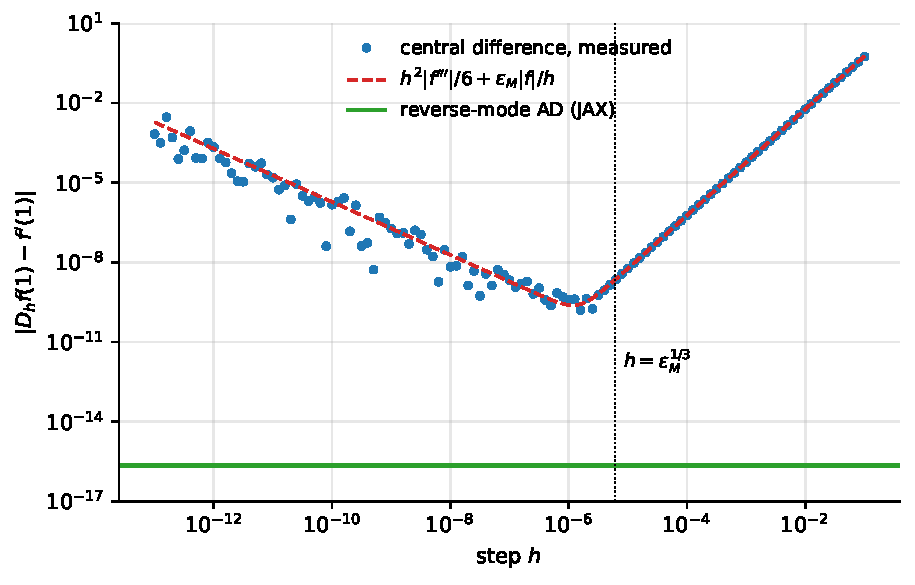
\includegraphics[width=0.75\textwidth]{BookFigures/chapter04_optimization/fd_vs_ad_error}
\caption{Absolute error of the central finite difference~(\ref{eq:4-centraldiff}) for $f(x)=\sin(2\pi x+x^{2})$ at $x=1$, as a function of the step $h$ (points), together with the model~(\ref{eq:4-fderror}) (dashed): truncation error $\propto h^{2}$ on the right, rounding error $\propto1/h$ on the left, and a minimum of about $10^{-10}$ near $h\approx\epsilon_M^{1/3}$.  The reverse-mode derivative computed by JAX has an error at the level of the unit roundoff, shown as the horizontal line, for any $h$ because it involves no $h$.}
\label{fig:4-fdvsad}
\end{figure}

The transformations of JAX compose: \texttt{jit(grad(f))} compiles the
gradient, \texttt{vmap(grad(f))} vectorises it over a batch,
\texttt{grad(grad(f))} differentiates it again and
\texttt{jvp(grad(f),\dots)} gives Hessian--vector products.  We shall use this
machinery freely from Chapter~\ref{chap:logreg} onwards, and in
Chapter~\ref{chap:nn} we shall meet reverse mode again under its older name.

%----------------------------------------------------------------------
\section{Practical tips}
\label{sec:practicaltips}

The following advice is collected from the sources cited in this chapter and
from experience; each item connects to something already derived.

\paragraph{Randomise the data when forming minibatches.}
Always shuffle before splitting into minibatches.  Otherwise the ordering of
the data becomes a systematic feature of the gradient sequence, and the method
can fit spurious correlations arising purely from the order of presentation.
If the data arrive sorted by class, an unshuffled minibatch may contain a
single class and its gradient will point somewhere unhelpful.

\paragraph{Transform your inputs.}
Learning is difficult when the landscape mixes steep and flat directions, and
Section~\ref{sec:learningrate} made that statement quantitative: the iteration
count scales with $\kappa$.  Standardising the inputs -- subtracting the mean
and dividing by the standard deviation, as in Section~\ref{sec:arrays} --
equalises the scales and reduces $\kappa$.  Whenever possible, decorrelate the
inputs as well.  The reason is exactly Eq.~(\ref{eq:1-hessian}): for a squared
error cost the Hessian \emph{is} the correlation matrix of the inputs, up to
normalisation, so standardising and decorrelating make the landscape as close
to spherical as it can be made, which by Eq.~(\ref{eq:4-gdrate}) is the
best case.  Since most deep networks are linear transformations followed by
non-linearities, the intuition carries beyond the linear case; this is also
the motivation for batch normalisation.

\paragraph{Monitor out-of-sample performance.}
Always track the cost on a validation set held out of training, as a proxy for
the test set of Section~\ref{sec:generalisation}.  When the validation error
begins to rise while the training error still falls, the model has started to
overfit and the run should be stopped.  This early stopping improves
performance substantially in many settings and costs nothing.

\paragraph{Adaptive methods do not always generalise well.}
As noted in Section~\ref{sec:adaptivecode}, several studies have found that
Adam, RMSProp and AdaGrad reach a worse test error than well-tuned SGD with
momentum, particularly when the number of parameters exceeds the number of
data points.  It is not settled why adaptive methods train deep networks so
effectively yet generalise less well; the practical conclusion is that a
properly tuned SGD may match or beat them, and is worth trying.

\paragraph{Check your gradients.}
Before trusting an optimiser, verify the gradient it is given.  Compare the
analytical expression against a central finite difference,
\begin{equation}
  \frac{\partial C}{\partial\theta_j}
   \approx \frac{C(\bm{\theta}+h\bm{e}_j)-C(\bm{\theta}-h\bm{e}_j)}{2h},
  \label{eq:4-gradcheck}
\end{equation}
with $h$ around $10^{-5}$, or against automatic differentiation.  An optimiser
given a wrong gradient does not usually crash; it quietly converges to the
wrong answer, which is far harder to detect.

\paragraph{Do not compare learning rates across optimisers.}
Table~\ref{tab:optimcompare} made the point: the same $\gamma$ means different
things to plain SGD and to Adam, because the latter has already normalised the
gradient.  Each method must be tuned on its own scale before any comparison is
meaningful.

%----------------------------------------------------------------------
\section{Summary and the programs}
\label{sec:ch4summary}

The chapter has one argument, developed in stages.

Minimising a cost function is easy when the cost is convex, because by
Section~\ref{sec:convexity} any stationary point is then a global minimum, and
the least-squares and Ridge problems of Chapter~\ref{chap:lreg} are convex.
Newton's method~(\ref{eq:4-newtonopt}) solves such problems ideally, in a
single step for a quadratic, and is invariant to how the parameters are
scaled.  It costs $\bigO(p^{3})$ per step and is therefore unavailable for
large models.

Gradient descent costs $\bigO(p)$ and pays for it in iterations.  The
decoupled error recursion~(\ref{eq:4-decoupled}) explained exactly why: the
step size is bounded above by $2/\lambda_{\max}$ for stability while progress
is governed by $\lambda_{\min}$, so the iteration count scales with the
condition number $\kappa$ of the Hessian -- and by
Eq.~(\ref{eq:4-kappasquared}) with the \emph{square} of the condition number
of the design matrix.  This single number connects the chapter to the two
before it: it is the quantity of Section~\ref{sec:norms} that governs
numerical accuracy, the quantity of Section~\ref{sec:olsstatistics} that
governs the variance of the fitted parameters, and now the quantity that
governs how long training takes.  Standardising features and adding a Ridge
penalty improve all three at once.

The remedies then form a sequence, each recovering a little more of what
Newton's method has and gradient descent lacks.  Momentum accumulates a
discounted history of gradients, amplifying consistent directions by
$1/(1-\beta)$ and cancelling oscillatory ones, which improves the rate from
$\kappa$ to $\sqrt{\kappa}$.  Stochastic gradients replace the full sum by a
minibatch, trading a worse rate per iteration for a far better rate per unit
of computation, and adding noise that helps escape poor local minima.  The
adaptive methods build a diagonal estimate of curvature from the second moment
of the gradient: AdaGrad by an unbounded sum, which eventually stalls; RMSProp
by an exponential moving average, which does not; and Adam by combining
RMSProp with momentum and correcting the initialisation bias with the factors
$1-\beta_i^{t}$ derived in Eq.~(\ref{eq:4-adambiasderiv}).

The demonstration of Table~\ref{tab:optimcompare} was deliberately
unflattering, and its two lessons should be kept.  A learning rate is not
comparable across optimisers, because the adaptive methods have already
normalised the gradient before $\gamma$ multiplies it.  And on a small, convex,
well-conditioned problem the adaptive machinery buys nothing and can cost a
great deal: these methods exist for large, ill-conditioned, non-convex
landscapes, which is where we shall meet them from Chapter~\ref{chap:logreg} onwards.

Finally, none of this is usable without gradients, and
Section~\ref{sec:autodiff} showed that they need not be derived by hand.
Automatic differentiation applies the chain rule to the evaluation trace of a
program: forward mode carries a tangent with every value and returns one
Jacobian--vector product per sweep, reverse mode carries an adjoint with
every node and returns one vector--Jacobian product per sweep, and by the
cheap gradient principle of Proposition~\ref{prop:4-cheapgradient} the latter
delivers the gradient with respect to all $p$ parameters for the price of a
few function evaluations, independent of $p$.  It is exact to rounding, where
finite differences are limited to $\epsilon_M^{2/3}$ by
Eq.~(\ref{eq:4-fdoptimal}), and it is the reason the models of the later
chapters can be written down at all.

The complete programs are collected in \texttt{doc/BookML/BookPrograms}:

\begin{itemize}
  \item \texttt{gradient\_descent.py} -- plain and momentum gradient descent on
        $f(x)=x^{2}$ and on the least-squares and Ridge problems of
        Section~\ref{sec:gdlinreg}, with the analytical solutions for
        comparison, and the empirical verification of the stability
        bound~(\ref{eq:4-stability}) and the rate~(\ref{eq:4-gdrate}).
  \item \texttt{stochastic\_gradient.py} -- minibatch SGD with a varying number
        of batches, the time-decay schedule~(\ref{eq:4-timedecay}), and a
        comparison of convergence per iteration against convergence per unit
        of computation.
  \item \texttt{adaptive\_optimizers.py} -- AdaGrad, RMSProp and Adam as in
        Section~\ref{sec:adaptivecode}, the learning-rate sweep of
        Table~\ref{tab:optimcompare}, and the same comparison repeated on a
        deliberately ill-conditioned design matrix where the adaptive methods
        win decisively.
  \item \texttt{autodiff\_examples.py} -- the \texttt{Dual} class of
        Section~\ref{sec:adforward}, the \texttt{autograd} and \texttt{JAX}
        versions of the least-squares and Ridge gradients, the explicit
        \texttt{jvp}/\texttt{vjp} and Hessian--vector products of
        Section~\ref{sec:adpython}, the four optimisers on the Rosenbrock
        function of Section~\ref{sec:adrosenbrock}, and the finite-difference
        error curve of Fig.~\ref{fig:4-fdvsad}.
\end{itemize}

Each file runs as a script and reproduces the numbers quoted in this chapter.
An executable version is available as a Jupyter notebook in the accompanying
Jupyter-book.

%=============================================================================
\section{Exercises}
\label{sec:ch4exercises}
%=============================================================================

\subsection*{Warm-up exercises}
\addcontentsline{toc}{subsection}{Warm-up exercises}

\begin{enumerate}

\item \textbf{Convexity from the definition.}
  Show that $f(x)=x^{2}$ is convex on $\mathbb{R}$ using
  Eq.~(\ref{eq:4-convexdef}).  Hint: show that
  $\lambda f(x)+(1-\lambda)f(y)-f(\lambda x+(1-\lambda)y)\ge0$ for all
  $x,y$ and $\lambda\in[0,1]$.

\item \textbf{Convexity from the second-order condition.}
  Using the second-order condition of Section~\ref{sec:convexity}, show that
  (a) $f(x)=e^{x}$ is convex on $\mathbb{R}$;
  (b) $g(x)=-\ln(x)$ is convex on $(0,\infty)$.

\item \textbf{Compositions.}
  Let $f(x)=x^{2}$ and $g(x)=e^{x}$.  Show that $f(g(x))$ and $g(f(x))$ are
  convex on $\mathbb{R}$.  Show more generally that if $f$ is any convex
  function then $h(x)=e^{f(x)}$ is convex.

\item \textbf{Norms are convex.}
  A norm satisfies $f(\alpha\bm{x})=|\alpha|f(\bm{x})$ and
  $f(\bm{x}+\bm{y})\le f(\bm{x})+f(\bm{y})$.  Using only these two properties
  and Eq.~(\ref{eq:4-convexdef}), show that a norm is convex.  Deduce that
  both the Ridge and the Lasso cost functions of Chapter~\ref{chap:lreg} are
  convex.

\item \textbf{The stability bound (numerical).}
  For the least-squares problem of Section~\ref{sec:gdlinreg}:
  (a) compute the eigenvalues of the Hessian~(\ref{eq:4-gdhessian}) and hence
      $\lambda_{\max}$, $\lambda_{\min}$ and $\kappa$;
  (b) run gradient descent for $\gamma$ just below and just above
      $2/\lambda_{\max}$ and confirm Eq.~(\ref{eq:4-stability});
  (c) measure the number of iterations needed to reach a fixed accuracy for
      several $\gamma$, and check that the minimum occurs near
      $\gamma^{*}=2/(\lambda_{\max}+\lambda_{\min})$.

\item \textbf{Conditioning and convergence (numerical).}
  Construct design matrices with condition numbers
  $\kappa_2(\bm{X})=10,10^{2},10^{3}$, for instance by rescaling the columns.
  (a) Measure the iteration count of gradient descent to fixed accuracy for
      each, and check the linear scaling with $\kappa$ predicted by
      Eq.~(\ref{eq:4-gdrate}).
  (b) Repeat with momentum and verify the $\sqrt{\kappa}$ scaling of
      Eq.~(\ref{eq:4-momentumrate}).
  (c) Repeat after standardising the columns, and comment.

\item \textbf{Momentum as a damped oscillator.}
  Consider the one-dimensional quadratic $C(\theta)=\tfrac{1}{2}\lambda\theta^{2}$.
  (a) Write the momentum update~(\ref{eq:4-momentum}) as a two-term recurrence
      in $\theta$.
  (b) Find the values of $\gamma$ and $\beta$ for which the recurrence has
      complex roots, and interpret them as oscillation.
  (c) Verify Eq.~(\ref{eq:4-momentumgain}) numerically by applying momentum to
      a constant gradient.

\item \textbf{Minibatch noise (numerical).}
  For a fixed $\bm{\theta}$, compute the minibatch gradient many times for
  batch sizes $M=1,4,16,64$ and measure the standard deviation of its
  components.  Verify the $1/\sqrt{M}$ scaling predicted by
  Section~\ref{sec:clt}, and discuss what it implies about the cost of
  reducing gradient noise.

\item \textbf{AdaGrad stalls (numerical).}
  Reproduce the $\gamma=0.01$ column of Table~\ref{tab:optimcompare}.
  (a) Plot the effective learning rate $\gamma/\sqrt{r_{t,j}}$ against $t$ for
      each coordinate and show that it decays towards zero.
  (b) Estimate the total distance the iterate can still travel after $t$
      steps, and compare with the distance remaining to the minimum.
  (c) Repeat with RMSProp and explain, using
      Eq.~(\ref{eq:4-rmspropsum}), why the decay does not occur.

\item \textbf{Adam's bias correction (numerical).}
  (a) Implement Adam with and without the bias
      correction~(\ref{eq:4-adambias}) and compare the first twenty steps.
  (b) For a constant gradient $g$, verify Eq.~(\ref{eq:4-adambiasderiv})
      numerically.
  (c) Show that with $\beta_2=0.999$ the uncorrected $\sqrt{v_1}$ is smaller
      than the true root mean square gradient by a factor of about $32$, and
      explain what that does to the first step.

\item \textbf{Dual numbers.}
  (a) Using only $\varepsilon^{2}=0$, derive the rules for the quotient
      $(a+b\varepsilon)/(c+d\varepsilon)$ and for $\sqrt{a+b\varepsilon}$, and
      check that they reproduce the quotient rule and $d\sqrt{x}/dx$.
  (b) Show from Eq.~(\ref{eq:4-dualtaylor}) that dual numbers cannot deliver
      second derivatives, and that the ``hyper-dual'' algebra with two
      symbols $\varepsilon_1,\varepsilon_2$, $\varepsilon_1^{2}=\varepsilon_2^{2}=0$
      but $\varepsilon_1\varepsilon_2\neq0$, can.
  (c) Extend the \texttt{Dual} class of Section~\ref{sec:adforward} with
      \texttt{sqrt} and \texttt{\_\_truediv\_\_} for a dual denominator, and
      verify your rules numerically.

\item \textbf{Forward and reverse sweeps by hand.}
  For $f(x_1,x_2)=x_1x_2+\exp(x_1x_2)-\sin x_1$ at $(x_1,x_2)=(1,2)$:
  (a) write down the evaluation trace and draw the computational graph, as
      in Eq.~(\ref{eq:4-adtrace}) and Fig.~\ref{fig:4-compgraph};
  (b) carry out the forward sweep~(\ref{eq:4-forwardrec}) for both
      coordinate directions;
  (c) carry out the reverse sweep~(\ref{eq:4-reverserec}) once, and confirm
      that it delivers both partial derivatives;
  (d) count the multiplications in (b) and in (c), and check the operation
      count against Proposition~\ref{prop:4-cheapgradient}.

\item \textbf{Reverse mode for least squares.}
  Write the least-squares cost~(\ref{eq:4-gdcost}) as the trace
  $\bm{v}_1=\bm{X}\bm{\theta}$, $\bm{v}_2=\bm{v}_1-\bm{y}$,
  $v_3=\bm{v}_2^{T}\bm{v}_2/n$, with vector-valued nodes.  Apply the reverse
  recursion~(\ref{eq:4-reverserec}) with the vector--Jacobian
  products~(\ref{eq:4-vjp}) of each stage, and show that it produces the
  gradient~(\ref{eq:4-gdgradient}) $\frac{2}{n}\bm{X}^{T}(\bm{X}\bm{\theta}-\bm{y})$
  without ever forming a Jacobian larger than $\bm{X}$ itself.  Explain why
  the adjoint $\bar{\bm{v}}_1$ is what Chapter~\ref{chap:nn} will call the
  output error.

\item \textbf{Hessian--vector products (numerical).}
  (a) Implement Eq.~(\ref{eq:4-hvp}) in JAX as forward-over-reverse,
      \texttt{jvp(grad(f))}, and alternatively as reverse-over-reverse,
      \texttt{grad(lambda x: grad(f)(x) @ v)}.  Check both against \texttt{jax.hessian}
      on the Ridge cost~(\ref{eq:4-ridgecost}).
  (b) Use only Hessian--vector products and the conjugate-gradient method to
      solve the Newton system~(\ref{eq:4-newtonopt}) for the Rosenbrock
      function~(\ref{eq:4-rosenbrock}), and reproduce the six-step
      convergence of Section~\ref{sec:adrosenbrock} without ever forming
      the Hessian.

\item \textbf{The finite-difference error curve (numerical).}
  Reproduce Fig.~\ref{fig:4-fdvsad} for $f(x)=e^{x}$ at $x=1$ and for
  $f(x)=\tan x$ at $x=1.5$.  From the measured minimum, estimate $\epsilon_M$
  and $|f'''|$ using Eq.~(\ref{eq:4-fdoptimal}), and compare with the true
  values.  Repeat in single precision (\texttt{np.float32}) and explain the
  change.

\end{enumerate}

%----------------------------------------------------------------------
\subsection*{Project-style exercise: optimisers on an ill-conditioned problem}
\addcontentsline{toc}{subsection}{Project-style exercise: comparing optimisers}

The comparison in Table~\ref{tab:optimcompare} was made on a problem too easy
to distinguish the methods.  The purpose of this exercise is to build one that
does, and thereby to see the arguments of this chapter operate.

\paragraph{Part a: build the landscape.}
Generate a polynomial regression problem from the Franke function of
Section~\ref{sec:franke}, or from a one-dimensional polynomial of degree ten
with the Vandermonde design matrix~(\ref{eq:3-vandermonde}).  Compute
$\kappa_2(\bm{X})$ and $\kappa_2(\bm{X}^{T}\bm{X})$ and confirm
Eq.~(\ref{eq:4-kappasquared}).  Then produce a second version with the columns
standardised and compare the two condition numbers.

\paragraph{Part b: plain gradient descent.}
Implement gradient descent with the analytical
gradient~(\ref{eq:4-gdgradient}).  Determine empirically the largest stable
$\gamma$ and compare with Eq.~(\ref{eq:4-stability}).  Plot the cost against
iteration for several $\gamma$ on both the raw and the standardised problem.

\paragraph{Part c: momentum and stochasticity.}
Add momentum and confirm the improvement in iteration count.  Then implement
minibatch SGD with the time-decay schedule~(\ref{eq:4-timedecay}), and compare
convergence per iteration and per gradient evaluation.  Which comparison is
the fair one, and why?

\paragraph{Part d: the adaptive methods.}
Implement AdaGrad, RMSProp and Adam.  For each, sweep $\gamma$ over several
orders of magnitude and record the best result; present the outcome as a table
like Table~\ref{tab:optimcompare}.  Discuss which methods are sensitive to
$\gamma$ and which are not, and relate your finding to whether the method
normalises the gradient before applying $\gamma$.

\paragraph{Part e: the diagonal approximation and its limits.}
Construct two problems with the same condition number, one whose Hessian is
diagonal and one whose narrow valley runs at $45$ degrees to the coordinate
axes -- the second is obtained from the first by an orthogonal rotation of the
features, which by Section~\ref{sec:orthogonal} leaves $\kappa$ unchanged.
Run all the methods on both.  Explain, using the final notebox of
Section~\ref{sec:adam}, why the adaptive methods help on the first and not on
the second, and what this says about the difference between a diagonal
approximation to $\bm{H}$ and the real thing.

\paragraph{Part f: automatic differentiation.}
Repeat part b using \texttt{autograd} or \texttt{JAX} instead of the
hand-derived gradient, and verify that the two agree to machine precision.
Then apply the gradient check~(\ref{eq:4-gradcheck}) and compare the accuracy
of the finite difference with that of automatic differentiation as $h$ is
varied over many orders of magnitude.  Explain the shape of the resulting
curve using the discussion of round-off error in
Section~\ref{sec:norms}.
